\documentclass[letter, 10pt]{article}
\usepackage[utf8]{inputenc}
%%\usepackage[spanish]{babel}
\usepackage{amsfonts}
\usepackage{amsmath}
\usepackage[dvips]{graphicx}
\usepackage{url}
\usepackage{ctable} % for \specialrule command
\usepackage[top=3cm,bottom=3cm,left=3.5cm,right=3.5cm,footskip=1.5cm,headheight=1.5cm,headsep=.5cm,textheight=3cm]{geometry}
\usepackage{lscape}
\usepackage{hyperref}
\usepackage[ruled,vlined, spanish, onelanguage]{algorithm2e}
\usepackage{float}
\usepackage{longtable}
\usepackage{etoolbox}
\patchcmd{\thebibliography}{\section*{\refname}}{}{}{}
\newcommand*\sq{\mathbin{\vcenter{\hbox{\rule{.7ex}{.7ex}}}}}

\begin{document}
\title{Inteligencia Artificial \\ \begin{Large}Estado del Arte: Examination Timetabling Problem\end{Large}}
\author{Gonzalo Fernández}
\date{\today}
\maketitle


%--------------------No borrar esta sección--------------------------------%
\section*{Evaluación}

\begin{tabular}{ll}
Resumen (5\%): & \underline{\hspace{2cm}} \\
Introducción (5\%):  & \underline{\hspace{2cm}} \\
Definición del Problema (10\%):  & \underline{\hspace{2cm}} \\
Estado del Arte (35\%):  & \underline{\hspace{2cm}} \\
Modelo Matemático (20\%): &  \underline{\hspace{2cm}}\\
Conclusiones (20\%): &  \underline{\hspace{2cm}}\\
Bibliografía (5\%): & \underline{\hspace{2cm}}\\
 &  \\
\textbf{Nota Final (100\%)}:   & \underline{\hspace{2cm}}
\end{tabular}
%---------------------------------------------------------------------------%
\vspace{2cm}


\begin{abstract}
El Examination Timetabling Problem (ETP) es un problema que consta de asignar horarios a un conjunto de exámenes bajo ciertas restricciones, la calidad de esta asignación tiene un gran impacto en el desempeño de los estudiantes a la hora de rendir sus exámenes, lo que hace de este un problema sumamente importante y estudiado a lo largo de la historia, pero que a su vez, se han identificado variantes según las necesidades de cada institución. Este documento plantea los orígenes del problema, cómo ha sido abordado en el tiempo, un modelo matemático y la aplicación de Forward Checking para su resolución, así como también, algunas conclusiones respecto al trabajo actual y futuro sobre el cual se deba guiar el resto de su investigación.
\end{abstract}

\section{Introducción}

Una de las herramientas más importantes para medir el conocimiento adquirido de un estudiante en cualquier institución educativa son los exámenes, de estos depende la aprobación de un curso y por lo tanto, mientras mejores condiciones se brinden para su rendición, mejores resultados pueden esperarse \cite{MUKLASON2019647}. Estas condiciones se dan por diversos factores, entre ellos están los horarios en que los exámenes son asignados pues un estudiante no puede rendir 2 exámenes al mismo tiempo y a su vez, necesita un tiempo de preparación entre exámenes. Asignar estos horarios es una tarea recurrente que consume mucho tiempo y se realiza comúnmente ajustando a la actualidad alguna asignación de exámenes previa, o bien con apoyo de un sistema de administración que no automatiza del todo el proceso \cite{NAJIAZIMI2005705}, no obstante ninguno de estos enfoques se sostiene ante la constante variación de cursos, estudiantes y otros factores a lo largo del tiempo, lo que hace de este un problema complejo y con mucha importancia dentro de una institución educativa.\\

A este problema se le conoce como Examination Timetabling Problem (ETP), el cual se define como "la calendarización de exámenes de un conjunto de cursos universitarios, evitando traslapes de cursos con estudiantes en común, y distribuyendo los exámenes de la mejor forma posible" \cite{Schaerf1999}. El ETP forma parte de la familia de problemas NP-completos \cite{10.1093/comjnl/10.1.85}, lo cual indica que no es posible resolver el ETP en un tiempo razonable. Por otro lado, se suma a esto que cada institución educativa cuenta con distintos requerimientos a la hora de asignar los horarios de sus exámenes, de estos requerimientos se distinguen 2 tipos de restricciones al problema \cite{Qu2009}, llamadas restricciones blandas (que deben satisfacerse lo mayor posible) y restricciones duras (que siempre deben ser satisfechas). Las restricciones duras deben ser satisfechas siempre, las blandas en cambio, deben satisfacerse lo mayor posible con el fin de lograr una mejor solución. En este documento se trabajará una variación donde se cuenta con un conjunto de exámenes y un conjunto de estudiantes que debe rendirlo, el objetivo será buscar una asignación de horarios tal que ningún estudiante tenga 2 exámenes al mismo tiempo y que a su vez, se minimice la cantidad de horarios necesarios para llevar a cabo los exámenes, un segundo objetivo menos importante será distribuir los exámenes lo mejor posible, de manera tal que los estudiantes cuenten con tiempo para estudiar entre cada examen, no obstante, éste último no es un objetivo más importante que el de disminuir la cantidad de horarios.\\

La NP-completitud del problema, sus variadas restricciones duras (ver Tabla~\ref{tab:duras}) y blandas (ver Tabla~\ref{tab:blandas}) y su enorme impacto tanto en el área de la educación como en problemas de horarios en general, hacen de este un problema sumamente interesante e importante de resolver.\\ 

El presente documento se estructura de la siguiente manera: primero se definirá el problema del ETP, se hablará sobre sus variantes y se detallará la variante a trabajar en la sección (\ref{definicion}); luego se dará una reseña histórica del problema a través de su estado del arte en la sección (\ref{estado}); luego se planteará un modelo matemático que permita resolver la variante del ETP que se está estudiando en la sección (\ref{modelo}); seguido de ésto se formulará una representación las soluciones del problema en la sección (\ref{representacion}); que luego será usada en la descripción de un algoritmo que resuelta el ETP en la sección (\ref{algoritmo}); luego se plantearán experimentos que hagan uso del algoritmo en la sección (\ref{experimentos}); seguido de ésto se presentarán los resultados obtenidos en la sección (\ref{resultados}); finalmente, se entregan algunas conclusiones sobre los contenidos tratados e ideas de trabajo a futuro sobre este problema en la sección (\ref{conclusiones}).

\section{Definición del Problema} \label{definicion}

El ETP es un Timetabling Problem, y como tal se compone de 4 parámetros principales: un conjunto finito de tiempos, un conjunto finito de recursos, un conjunto finito de reuniones y un conjunto finito de restricciones \cite{Qu2009}, donde en su forma más general los tiempos son los horarios en que se toman los exámenes, los recursos serían los estudiantes y las salas en donde estos se llevan a cabo, las reuniones serían los exámenes que cuentan con estudiantes que deben rendirlos y el conjunto de restricciones sería que un estudiante no puede tener asignado 2 o más exámenes al mismo tiempo, entre otras, buscando así generar una asignación de horarios a los exámenes tal que se satisfagan lo mejor posible las restricciones. Ésta definición general permite abordar el ETP como un problema de búsqueda ya que bastaría con satisfacer las restricciones duras (ver Tabla~\ref{tab:duras}) del problema como lo sería que un estudiante no tenga 2 exámenes al mismo tiempo, no obstante, las necesidades de las instituciones educacionales van requieren considerar un conjunto de restricciones blandas(ver Tabla~\ref{tab:blandas}), las cuales hacen de este problema uno de optimización por sobre uno de búsqueda.\\

Las variaciones a este problema corresponden a la realidad de cada institución educacional en la que el autor se concentra a la hora de estudiarlo, entre estas se encuentran la implementación de diversas versiones para el mismo examen, de modo tal que un estudiante no tenga 2 exámenes al mismo tiempo y así, mejorar la distribución de los mismos \cite{WOUMANS2016178}, otra variación considera un subconjunto de salas para cada examen donde éste puede ser rendido y consultar a los estudiantes sus preferencias para calendarizar evaluaciones, sin que ésto les garantice que serán calendarizadas en esos horarios \cite{LAPORTE1984351}. Todos estos ajustes hacen de este un problema lleno de variaciones en la práctica (no así en los benchmarks donde se ocupan datasets específicos como por ejemplo el ITC2007 \cite{ITC2007}), más no hay una variación particular en la que la literatura se concentre.\\

Al ser un Timetabling Problem, todos los problemas de esta familia se parecen en cierta medida al ETP, pero los que más parecidos son el Timetabling Course Problem que consta de asignar un conjunto de cursos a un conjunto finito de horarios y salas; y el School Timetabling Problem que consta de asignar un conjunto de distintos recursos (horarios, profesores, estudiantes, salas, etc) a un conjunto de eventos \cite{TAN2021113943}, ambos han sido ampliamente estudiados y sus descubrimientos han aportado mútuamente tanto al ETP como a otros Timetabling Problems.

Para efectos de este documento, se trabajará la siguiente variante: Se cuenta con un conjunto de exámenes y un conjunto de estudiantes que debe rendirlos, el objetivo será asignar la menor cantidad posible de horarios de exámenes tal que ningún estudiante tenga 2 exámenes al mismo tiempo y, en el camino, intentar distribuir los exámenes lo más posible para así aumentar el tiempo entre exámenes de cada estudiante, no obstante, el objetivo principal será disminuir la cantidad de horarios con los cuales llevar a cabo los exámenes.

\section{Estado del Arte} \label{estado}

Las primeras apariciones del ETP en la literatura datan del 1964, donde Broder \cite{10.1145/355586.364824} da una formalización del problema debido a la necesidad de asignar los horarios de los exámenes finales de los cursos de una universidad y propone un modelo matemático para el mismo, también propone un algoritmo aleatorizado de tipo Monte Carlo para encontrar una solución que minimizara la cantidad de conflictos entre estudiantes y sus exámenes, esta solución encontrada si bien no garantizaba ser la mejor, usualmente sería óptima. Ese mismo año Cole \cite{10.1093/comjnl/7.2.117} propone una matriz de conflictos entre exámenes y una serie de restricciones particulares, junto con un algoritmo ``largest degree first: fill from top'' para generar una solución que también sería cercana a la óptima, además su método puede ejecutarse en computadores con poca capacidad de almacenamiento.\\ 

En 1966, Peck \cite{10.1145/365696.365713} propone un algoritmo de particionamiento y coloreo de grafos el cual sólo se encarga de asignar horarios lo mejor posible sin garantizar que un estudiante no tendrá 2 exámenes al mismo tiempo ni considerar otras restricciones. Ya en 1968, Wood \cite{10.1093/comjnl/11.1.41} ideó un algoritmo que fue implementado en su universidad, éste también se basó en la minimización de una matriz de conflictos como la de Cole \cite{10.1093/comjnl/7.2.117}, no obstante, la calidad de la solución que éste entregaba se medía según los criterios de aquella universidad, por otro lado, en caso de que 2 cursos empatasen en su asignación, Wood implementó una estrategia ``look ahead'' para elegir qué examen sería asignado en ese horario, de modo tal que esta decisión no generara problemas en las próximas asignaciones y en caso de no poder entregar una asignación completa, bastaba con asignar manualmente los cursos que no quedaron asignados y echar a andar de nuevo el algoritmo, no obstante, dado el crecimiento exponencial de memoria que sufre al aumentar el tamaño de la entrada, éste algoritmo puede usarse con todos los exámenes de una universidad al mismo tiempo, requiere separar su uso en unidades lógicas como por ejemplo las carreras o departamentos.\\ 

Más adelante, Desroches et. al. \cite{11731709} presentan en 1978 el algoritmo HOREX, el cual es descrito en sus distintas etapas donde usa desde algoritmos de coloreo de grafos hasta programación entera para resolver el problema, resultando ser un algoritmo superior a los anteriores para una cantidad pequeña de horarios disponibles para realizar la asignación, pero no estando a la altura para escenarios más grandes. Un año más tarde White y Chan \cite{155986.1979.11731735} desarrollaron un algoritmo derivado de HOREX para aplicarlo en su universidad, buscando mejorar la satisfacción de restricciones blandas, no obstante, su buen desempeño también se veía restringido a cantidades pequeñas de horarios para realizar la asignación.\\ 

En 1981 Mehta \cite{10.2307/25060145} hizo un método (también para su universidad) cuyo fin era minimizar los conflictos y los casos en que 3 exámenes seguidos eran asignados, utilizando un enfoque de coloreo de grafos y una rutina de ``compresión'' para computar los conflictos que podía generar una asignación y escoger qué horario eliminar de ésta para volver a distribuir los exámenes, sus resultados fueron un gran aporte para demostrar que los ``saturation degree methods'' son las mejores técnicas de coloreo de grafos, respaldando a su vez las técnicas previas y marcando un punto en que encontrar soluciones libres de conflictos para este problema ya era una realidad.\\

Ya en 1984, Laporte et. al. \cite{LAPORTE1984351} presentaron el sistema HORHEC donde por primera vez se planteó la idea del ``costo de aversión'' basado en una lista de preferencias de los estudiantes y el ``costo de proximidad'' basado en la cantidad de horarios entre los cuales son asignados 2 exámenes, éstas restricciones blandas se sumarían a la restricción dura de no asignar más de 1 examen al mismo tiempo para 1 mismo estudiante (entre otras). La estrategia que plantearon se encargaba de probar la generación de asignaciones de horarios buscando minimizar la función objetivo planteada, aumentando la cantidad máxima de horarios a usar según un mínimo y máximo indicados por el usuario, ésta estrategia podría verse como un un polynomially bounded backtracking que permite ``corregir errores anteriores'' de soluciones previas \cite{10.2307/170814}, siendo así de los primeros algoritmos en no presentar una heurística de coloreo de grafos por detrás como los anteriores para resolver el problema.\\

Pese a estos avances, la mayoría de las soluciones propuestas se concentraban en el contexto de la institución educacional particular de los autores, sin que éstas llegasen a ser usadas en otras instituciones con realidades distintas, tampoco se realizaron comparaciones entre éstas y otros enfoques alternativos, en el fondo, la mayoría de autores no estaban al tanto de la existencia de otras soluciones publicadas debido a un muy desorganizado estado del arte \cite{10.2307/170814} hasta que en 1996, Carter et. al. \cite{10.2307/3010580} estudiaron 5 de las estrategias previamente mencionadas concluyendo que ninguna de ellas era sobresaliente para todos los casos en los que fueron probadas, no obstante, introdujeron al estudio de este problema un conjunto de 13 casos de prueba para así realizar benchmarks y dar un primer paso a estandarizar las comparaciones \cite{Qu2009}. Desde entonces, es posible comenzar a organizar de mejor manera las soluciones que se han propuesto.

\subsection*{Técnicas Basadas en Satisfacción de Restricciones}

Debido a la flexibilidad con la que estas técnicas se podían aplicar al ETP, se propusieron métodos de satisfacción de restricciones para resolver el problema, no obstante, debido al crecimiento exponencial de memoria que requieren, en su mayoría sólo podían generar soluciones parciales, que luego requerían ser completadas o mejoradas por otros procedimientos \cite{10.1007/BFb0055888, 10.1007/978-3-540-45157-0_14, ahnkim}, aunque también habían casos en que se ajustaban perfectamente a las necesidades de la universidad donde se implementaban \cite{tacadaograce}. Estas técnicas fueron respaldadas por grandes avances en lenguajes de programación de restricciones, pero no lograron ser un enfoque superior a la hora de aplicarse al problema de manera general, si no más bien, se ajustaban a las realidades de la universidad correspondiente, aunque es importante destacar que para ciertos casos de prueba, logran los mejores resultados \cite{Qu2009}.

\subsection*{Técnicas de Búsqueda Local}

Estas técnicas se guiaban por el uso de una función objetivo que permitía evaluar la calidad de las soluciones generadas y permitían manejar fácilmente las diferentes restricciones de las variantes del ETP. Entre estas podemos encontrar Tabu Search, donde se implementaron funciones objetivo adaptativas \cite{10.1007/3-540-44629-X_7}, búsquedas por fases (en cada fase de búsqueda de la solución se añaden restricciones no consideradas antes) y asignación de prioridades a las restricciones \cite{paquetehmm}.\\ 

Otra técnica usada es Simulated Annealing, la cual por sí sola no generaba soluciones mejores que otros métodos, no obstante, entonces se investigó el usarlo de forma híbrida con backtracking \cite{THOMPSON1998637}, obteniendo resultados mucho mejores e incentivando así el uso de enfoques que usaran esta técnica de forma híbrida. Merlot \cite{10.1007/978-3-540-45157-0_14} reforzó esta idea y realizó un híbrido con técnicas de programación de restricciones, logrando así los mejores resultados conocidos hasta la época y marcando un precedente para los enfoques híbridos a la hora de atacar el ETP.\\

Otros autores enfocaron su investigación en modificar la estructura de los vecindarios de búsqueda del espacio de soluciones a la hora de abordar el ETP , no obstante, el enorme cómputo que requieren las deja muy por detrás de las otras soluciones \cite{Qu2009}

\subsection*{Algoritmos Basados en Población}

Entre los algoritmos basados en población se trabajaron algoritmos de hormigas para resolver el modelo del ETP planteado como un problema de coloreo de grafos \cite{hormigasowo}, sin considerar restricciones blandas ni obtener resultados significativos en comparación con los demás. También se trabajaron algoritmos genéticos y meméticos con el fin de determinar las mejores heurísticas para resolver el problema \cite{10.1007/3-540-44629-X_9, niche, sheibani2002evolutionary}, así como también, encontrar la mejor representación del problema con el fin de mejorar los resultados, no obstante, las soluciones por éste ámbito no destacan tanto como las otras. También se trabajó con Artificial Immune Algorithms \cite{malim2006artificial}, los cuales presentaron los mejores resultados en ciertos casos de prueba, demostrando así el potencial de estos algoritmos para trabajos futuros con ellos \cite{Qu2009}.

\subsection*{Técnicas Multi-Criterio}

Con el fin de cuantificar la calidad de una solución bajo un criterio distinto al de calcular una función objetivo, se plantearon técnicas multi-criterio las cuales \cite{10.1093/comjnl/7.2.117, 10.1007/3-540-44629-X_8}, si bien entregaron buenos resultados en ciertos casos, su aporte al problema fue brindar flexibilidad para determinar la importancia individual de cada restricción con el fin de obtener soluciones deseadas más allá de las que minimizaban una función objetivo particular.

\subsection*{Técnicas Basadas en Grafos}

Distintos autores introdujeron mejoras en las heurísticas de coloreo de grafos para atacar el problema \cite{Burke98asimple, Scheduling_solvingexamination} e integrando técnicas de redes neuronales para generar mejores soluciones \cite{10.1007/11844297_40}, estas técnicas híbridas generaron buenos resultados usando los datasets actuales, por lo que más adelante dan pie al uso de hyperheurísticas más adelante. 

\subsection*{Técnicas de Descomposición y Clustering}

También se trabajó la idea de descomponer el problema en pequeños subproblemas \cite{notfoundxd, 752921} para encontrar soluciones óptimas, no obstante, el gran problema de este enfoque es que no se pueden evaluar restricciones blandas cuando un problema es descompuesto, por lo que no generó mucho impacto pese a lograr uno de los mejores resultados para 1 sólo caso de prueba \cite{burkeadaptative}

\subsection*{Hyperheurísticas}

Dada la dificultad de encontrar meta-heurísticas que se ajusten a las variaciones que puede un ETP particular tanto en sus restricciones blandas~\ref{tab:blandas} y duras~\ref{tab:duras}, por lo que se desarrollaron hyperheurísticas con resultados prometedores para fomentar futuras investigaciones usando esta técnica \cite{prosss}, dando como resultado que para el 2019 se planteara una hyperheurística basada en el algoritmo Great Deluge, cuyos resultados fueron sobresalientes en todos los casos de prueba usados en comparación a otras técnicas \cite{MUKLASON2019647}, posicionándose como una de las mejores técnicas hasta el momento y sentando las hyperheurísticas como las bases para trabajos futuros.

\begin{table}[]
\centering
\resizebox{\textwidth}{!}{%
\begin{tabular}{lp{13.45cm}}
\hline
   & Principales restricciones duras \\ \specialrule{.1em}{.05em}{.05em} 
1. & Los exámenes no deben compartir recursos (por ejemplo, estudiantes) de manera simultánea\\
2. & Los recursos deben ser suficientes (es decir, el número de estudiantes asignados a una sala debe ser menor o igual a la capacidad de la misma, así como también, deben haber suficientes salas para todos los exámenes) \\ \hline
\end{tabular}%
}
\caption{Principales restricciones duras en ETP \cite{Qu2009}}
\label{tab:duras}
\end{table}

\begin{table}[]
\centering
\resizebox{\textwidth}{!}{%
\begin{tabular}{lp{13.45cm}}
\hline
 	& Principales restricciones blandas \\ \specialrule{.1em}{.05em}{.05em} 
1. 	& Distribuir los exámenes que entran en conflicto de la manera más uniforme posible, o bien, no en x horarios consecutivos o días \\
2. 	& Grupos de exámenes que requieren ser tomados al mismo tienpo, en el mismo día o en el mismo lugar. \\
3. 	& Exámenes que deben ser consecutivos. \\
4. 	& Calendarizar todos los exámenes, o los más largos, lo antes posible. \\
5. 	& Un ordenamiento (precedencia) de exámenes necesita ser satisfecha. \\
6. 	& Número limitado de estudiantes y / ó exámenes en cierto horario. \\
7. 	& Requerimientos de tiempo (por ejemplo, realizar (o no) exámenes en ciertos horarios). \\
8. 	& Exámenes que entran en conflicto en el mismo día deben ser asignados en horarios cercanos. \\
9. 	& Exámenes que pueden separarse sobre distintos lugares. \\
10. & Sólo exámenes del mismo largo pueden ser asignados en la misma sala. \\
11. & Requerimientos de recursos (por ejemplo, salas con facilidades específicas para el examen). \\ \hline
\end{tabular}%
}
\caption{Principales restricciones blandas en ETP \cite{Qu2009}}
\label{tab:blandas}
\end{table}


\section{Modelo Matemático} \label{modelo}

Con el fin de resolver la variante del ETP a trabajar, se propone un modelo matemático que considera un costo de proximidad entre exámenes \cite{LAPORTE1984351} y que busca minimizar la cantidad de horarios \cite{WIJGERS}\\

\textbf{Parámetros:}

\begin{itemize}
	\item[$\sq$] $E$: Cantidad de exámenes, con $E \geq 1$
	\item[$\sq$] $L$: Cantidad máxima de horarios, con $L \geq 1$
	\item[$\sq$] $e_i$: Cantidad de estudiantes que deben rendir el examen $i$, con $1 \leq i \leq E$
	\item[$\sq$] $C_{ij}$: Cantidad de estudiantes que deben rendir el examen $i$ y $j$, con ($1 \leq i < j \leq E$)
	\item[$\sq$] $w_{s}$: Costo de proximidad entre exámenes separados por $s$ horarios
	\begin{itemize}
		\item[] Se define según Laporte \cite{LAPORTE1984351} como: $w_{1} = 16, w_{2} = 8, w_{3} = 4, w_{4} = 2, w_{5} = 1$ 
	\end{itemize}

\end{itemize}

\textbf{Variables:}
\begin{itemize}
	\item[$\sq$] $x_{il} =
					\left\{
						\begin{array}{ll}
							1  & \mbox{si el examen } i \text{ es asignado en el horario } l \text{, con } \text{, con } 1 \leq i \leq E \text{ y } 1 \leq l \leq L \\
							0 & \mbox{en cualquier otro caso}
						\end{array}
					\right.$
	\item[$\sq$] $t_{l} =
					\left\{
						\begin{array}{ll}
							1  & \mbox{si el horario } l \text{ es usado en la solución, con } 1 \leq l \leq L \\
							0 & \mbox{en cualquier otro caso}
						\end{array}
					\right.$

	\item[$\sq$] $M$: Un número arbitrariamente grande ($M > C_{ij}; i, j = 1, \ldots ,E$, con $i < j$)
\end{itemize}

\textbf{Función Objetivo:}

\begin{equation} \label{eq:1}
	\text{min } F: \sum_{l=1}^{L} \sum_{s=1}^{5} \sum_{i=1}^{E} \sum_{j=1}^{E} (x_{il}x_{j,l-s} + x_{il}x_{j,l+s}) C_{ij} w_{s} + \sum_{l=1}^{L} t_{l}
\end{equation}

\textbf{Restricciones:}

\begin{equation} \label{eq:2}
	x_{il} + x_{jl} \leq 2 - \frac{C_{ij}}{M} \quad \forall i, j : i<j \wedge i, j \in \{1, \ldots, E\} \wedge l \in \{1, \ldots, L\}
\end{equation}

\begin{equation} \label{eq:3}
	\sum_{l=1}^{L} x_{il}t_l = 1 \quad \forall i \in \{1, \ldots, E\}
\end{equation}

\begin{equation} \label{eq:4}
	\sum_{i=1}^{E} \sum_{l=1}^{L} x_{il}t_l \leq L
\end{equation}

\textbf{Naturaleza de las Variables:}
\begin{equation*}
	x_{ij} \in \{1, 0\}
\end{equation*}

\begin{equation*}
	t_{l} \in \{1, 0\}
\end{equation*}

\begin{equation*}
	M \in \mathbb N
\end{equation*}

\textbf{Detalles del Modelo:}

\begin{itemize}
	\item[$\sq$] Dado que la minimización de los horarios a usar para la asignación es más importante que minimizar el costo de proximidad entre exámenes, el modelo plantea el parámetro $L$ para asignar el máximo de horarios que la institución educacional desea usar, el valor común para este parámetro debería ser $E$ poniéndose en el caso de que cada examen se asigne en un horario distinto y continuo.

	\item[$\sq$] La ecuación (\ref{eq:1}) es la función objetivo que mide la calidad de la solución y que el modelo busca minimizar, la primera parte de la sumatoria cuantifica el costo de proximidad entre exámenes mientras que la segunda parte cuantifica el costo asociado a la cantidad de horarios que se utilizarán.
	
	\item[$\sq$] La ecuación (\ref{eq:2}) busca que si un estudiante debe rendir los exámenes $i$ y $j$, entonces esos exámenes no pueden ser asignados en el mismo horario, la variable $M$ está para que si $C_{ij} > 0$ entonces la restricción sea equivalente a $x_{il} + x_{jl} \leq 1$ \cite{LAPORTE1984351}.

	\item[$\sq$] La ecuación (\ref{eq:3}) se asegura que un examen pertenezca a sólo 1 horario de los que se usarán en la solución (por eso considera $t_{l}$).

	\item[$\sq$] La ecuación (\ref{eq:4}) se asegura que no se asignen más de $L$ horarios (el máximo indicado por la institución educacional), para así evitar que se asigne una cantidad enorme de horarios con el fin de minimizar el costo de proximidad entre exámenes.

	\item[$\sq$] El espacio de búsqueda de este modelo matemático equivale a todas las combinaciones posibles de valores que se pueden realizar con las variables, lo que se expresa como $2^{(E + 1)L}$ y que determina el crecimiento exponencial del espacio de búsqueda en función de la cantidad de exámenes $E$ a asignar y la cantidad máxima de horarios $L$ que la institución educacional determina usar.
\end{itemize}

\section{Representación} \label{representacion}

La representación de las soluciones que se usará en los algoritmos descritos en la siguiente sección consta de una lista $s$ de tamaño $E$ (cantidad de exámenes), donde $s$[$i$] corresponde al horario asignado al examen $i$ para la calendarización. Ésta representación tiene un espacio de búsqueda de $E^{E}$ (se considera un máximo de $E$ horarios ya que siempre es posible encontrar una solución con ésta cantidad), el cual es mucho mejor que usar una matriz binaria $s_{E \times E}$ donde $s$[i][j] es 1 si el examen $i$ está asignado al horario $j$ y 0 si no, pues ésta tiene un espacio de búsqueda de $2^{2E}$. Además, ésta representación permite definir una cota superior $maxSlots$ a los horarios asignables que aumenta durante la ejecución del problema (ver \textit{Algoritmo 1}) y, a su vez, acota el espacio de búsqueda a recorrer de cada Backtracking realizado por una llamada al \textit{Algoritmo 2}. Otra ventaja de ésta representación es que permite definir una cota inferior $minSlots$ igual a la máxima cantidad de exámenes que un estudiante debe rendir. Al inicializar $maxSlots$ como $minSlots$, el Backtracking del \textit{Algoritmo 2} recorrerá un espacio de búsqueda de $(E-\text{minSlots})^{E}$ que luego crecerá según $\text{maxSlots}^{E}$ a medida que $maxSlots$ aumenta. Finalmente, la representación puede caer tanto en espacios factibles como infactibles, pues no filtra el espacio de búsqueda infactible del problema ni ayuda a cumplir restricciones de conflictos entre exámenes, no obstante, evita que un examen esté asignado en más de un horario a la vez. El siguiente diagrama muestra cómo funciona la representación (notar que la posición 0 de $s$ no se usa):

\begin{figure}[H]
\begin{center}
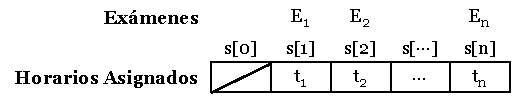
\includegraphics[width=0.5\textwidth]{img/s2.pdf}
\end{center}
\caption{Representación gráfica de una solución utilizando $s$.}
\label{fig:s1}
\end{figure}

Por ejemplo, para la siguiente instancia de 3 estudiantes con 3 exámenes:

\begin{figure}[H]
\begin{center}
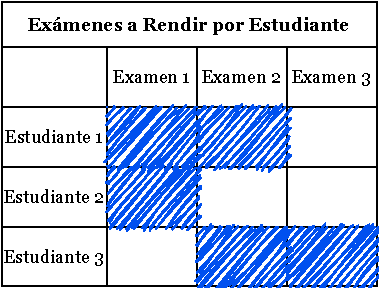
\includegraphics[width=0.4\textwidth]{img/s3.pdf}
\end{center}
\caption{Instancia de 3 exámenes y 3 estudiantes, los cuadros azules representan que el estudiante $i$ debe rendir el examen $j$.}
\label{fig:s2}
\end{figure}

La solución óptima puede expresarse como:

\begin{figure}[H]
\begin{center}
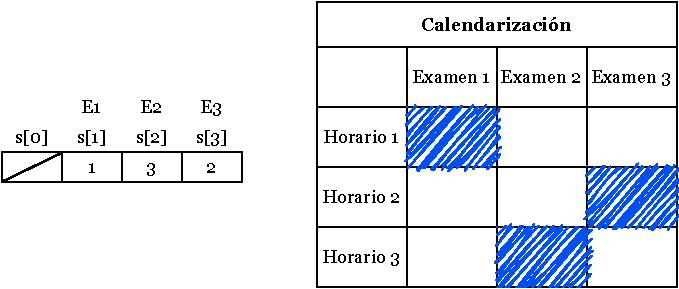
\includegraphics[width=0.7\textwidth]{img/s4.pdf}
\end{center}
\caption{Solución de la instancia representada en la Figura \ref{fig:s2}. Los cuadros azules denotan que el horario $i$ fue asignado al examen $j$.}
\label{fig:s3}
\end{figure}

\section{Descripción del Algoritmo} \label{algoritmo}

Para llevar a cabo la resolución del problema, se implementó un algoritmo de búsqueda completa con Forward Checking \cite{forwardchecking}. El algoritmo consiste en fijar una cantidad de horarios inicial a asignar entre el total de exámenes y, en caso de detectar que no es posible generar una calendarización válida con la cantidad de horarios fijadas, repetir el proceso considerando un horario extra. Cada vez que se asigna un horario a un examen, se lleva a cabo un filtro en los posibles horarios a asignar de los exámenes posteriores, es decir, se aplica arco-consistencia sin propagación entre la solución parcial y los dominios de los exámenes restantes. Si durante éste proceso un examen queda sin horarios disponibles para asignarle (vale decir, su dominio queda vacío), entonces se vuelven a agregar los horarios filtrados previamente y se intenta asignar el siguiente horario disponible al examen anterior, repitiendo el proceso. Cuando la cantidad de horarios a asignar es suficiente como para encontrar una calendarización válida, el algoritmo toma esa cantidad como la mínima necesaria para resolver la instancia y, sobre ella, intenta minimizar la penalización promedio asociada al esparcimiento de los exámenes asignados a cada estudiante.\\

Para facilitar las cosas, el algoritmo considera que el máximo de horarios siempre será la cantidad total de exámenes, pues en el peor de los casos, siempre será posible generar una calendarización válida asignando un horario distinto a cada examen (ejemplo, una instancia donde al menos 1 estudiante debiese rendir todos los exámenes). Además, se considera que el mínimo de horarios para comenzar la búsqueda completa debe ser la cantidad máxima de exámenes a rendir por algún estudiante, pues éste requerirá como mínimo 1 horario distinto por cada uno de sus exámenes. Finalmente, para la ejecución del algoritmo, se requiere contar con los siguientes parámetros y variables:

\begin{itemize}
	\item[$\sq$] \textbf{Parámetros}:
	\begin{itemize}
		\item[$\sq$] $E \leftarrow$ Cantidad de Exámenes
		\item[$\sq$] $L \leftarrow$ Cantidad máxima de exámenes que un alumno tiene asignado en la instancia, lo que a su vez, se considera la cantidad mínima de horarios para partir
		\item[$\sq$] $cMatrix_{E \times E} \leftarrow$ Matriz de conflictos entre exámenes, $cMatrix$[$i$][$j$] es 1 si el examen $i$ tiene conflictos con el examen $j$, 0 si no
	\end{itemize}
	\item[$\sq$] \textbf{Variables}:
	\begin{itemize}
		\item[$\sq$] $D$[$E$][$E$] $\leftarrow$ Lista de horarios asignables (dominio) del examen $i$, donde $D$[$i$][$j$] se marca con el examen del cual se realizó el FC para filtar el horario $j$
		\item[$\sq$] $s$[$E$] $\leftarrow$ Lista que representa la solución actual, donde $s$[$i$] almacena el horario asignado al examen $i$
		\item[$\sq$] maxSlots $\leftarrow$ Cantidad máxima de horarios a usar, se ajusta luego de cada BT + FC
		\item[$\sq$] minSlotsFound $\leftarrow$ Flag que indica si se encontró el mínimo de horarios necesarios para resolver la instancia
		\item[$\sq$] bestSol[E] $\leftarrow$ Mejor solución encontrada hasta el momento, misma representación que $s$[$i$]
		\item[$\sq$] bestPenalty $\leftarrow$ Penalización asociada a la mejor solución encontrada hasta el momento
	\end{itemize}
\end{itemize}

Teniendo esta información, el \textit{Algoritmo 1} ejecuta el \textit{Algoritmo 2} desde el primer examen para explorar el espacio de búsqueda considerando la mínima cantidad de horarios necesaria. Cuando termina su recorrido, si no se encuentra una solución que marque el flag $minSlotsFound$, se aumenta la cantidad mínima de horarios en 1 y se reinician los dominios filtrados de todos los exámenes para así repetir el proceso, según el siguiente algoritmo:\\

\begin{algorithm}[H]
\SetAlgoLined
\SetKwRepeat{Repeat}{Repeat}{Until}
\SetKwFunction{doBackTracking}{doBackTracking}
\SetKwFunction{doMaxTimeSlotsAdjustment}{doMaxTimeSlotsAdjustment}
\SetKwFunction{resetDomains}{resetDomains}
\KwResult{Encontrar una solución a una instancia del ETP con la mínima cantidad de slots}
\SetKwProg{maxSlotsAdjusment}{Procedure}{}{End}
\maxSlotsAdjusment{\doMaxTimeSlotsAdjustment{}}{
	maxSlots $\leftarrow $ 0\;
	bestPenalty $\leftarrow$ INF;
	\Repeat{minSlotsFound}{
		maxSlots $\leftarrow $ maxSlots + 1\;
		\doBackTracking{1}\;
		\resetDomains{0}\;
	}
}
\caption{Resolución del ETP con BT + FC aumentando la cantidad de horarios a usar}
\end{algorithm}

\vspace*{0.4cm}
Para recorrer el espacio de búsqueda se realiza un Backtracking recursivo que asigna un horario a cada examen en la lista $s$[examen]. Ésta asignación se lleva a cabo a partir de un examen al cual se asigna cada uno de los horarios disponibles en orden ascendente, siempre y cuando el horario no se encuentre filtrado del dominio del examen actual. Una vez asignado un horario válido al examen, se revisa si el examen trabajado es el último de la instancia, en tal caso se llegó a una solución factible con cantidad mínima de horarios necesaria para la calendarización, luego se marca el flag $minSlotsFound$ como verdadero y se calcula la penalización asociada. Ésta es la única parte del algoritmo donde se calcula la penalización pues no se puede calcular una penalización promedio coherente si no está toda la calendarización hecha. Si la penalización es menor a la penalización de la mejor calendarización encontrada hasta el momento, se actualiza $bestSol$ y $bestPenalty$, de lo contrario, se realiza arco consistencia entre la solución parcial y el resto de exámenes por asignar a través del \textit{Algoritmo 4}, que aplica la técnica de Forward Checking. Si el \textit{Algoritmo 4} indica que algún examen quedó sin horarios disponibles, entonces se reinician los dominios de los exámenes posteriores con el \textit{Algoritmo 3} y se intenta asignar el siguiente horario al examen actual, de lo contrario, se repite de manera recursiva el proceso para el examen posterior y al llegar a alguna hoja se reinician los dominios de los exámenes posteriores\\

\begin{algorithm}[H]
\SetAlgoLined
\SetKwFunction{doBackTracking}{doBackTracking}
\SetKwFunction{doMaxTimeSlotsAdjustment}{doMaxTimeSlotsAdjustment}
\SetKwFunction{checkSolution}{checkSolution}
\SetKwFunction{resetDomains}{resetDomains}
\SetKwFunction{calculatePenalty}{calculatePenalty}
\KwResult{Calendarización de exámenes para la cantidad de horarios actual, o bien, determinar que no es posible una calendarización con la cantidad de horarios disponible}
\SetKwProg{backtracking}{Procedure}{}{End}
	\backtracking{\doBackTracking{exam}}{
	slot $\leftarrow 1$\;
	\While{slot $\leq$ maxSlots}{
		\If{D[exam][slot]}{continue}
		s[exam] $\leftarrow$ slot\;
		\uIf{exam es el último examen por asignar}{
			minSlotsFound $\leftarrow true$\;
			penalty = \calculatePenalty{s}\;
			\If{bestPenalty $<$ penalty}{
				bestSol = s\;
				bestPenalty = penalty\;
			}			
		} \Else {
			\If{doForwardChecking() retorna 0}{
				\resetDomains{exam}\;
				continue\;
			}
			\doBackTracking{exam + 1}\;
			\resetDomains{exam}\;
		} 
		slot $\leftarrow$ slot + 1\;
	}
 }
 \caption{Asignar un horario a cada examen filtrando los horarios disponibles con Forward Checking}
\end{algorithm}
\vspace*{0.4cm}

\begin{algorithm}[H]
\SetAlgoLined
\SetKwRepeat{Repeat}{Repeat}{Until}
\SetKwFunction{resetDomains}{resetDomains}
\KwResult{Reiniciar (marcar con 0) los dominios filtrados por la arco-consistencia aplicada por el Forward Checking desde el examen indicado}
\SetKwProg{maxSlotsAdjusment}{Procedure}{}{End}
\maxSlotsAdjusment{\resetDomains{actualExam}}{
	exam $\leftarrow$ actualExam + 1\;
	\While{exam $\leq$ E}{
		horario $\leftarrow$ 1\;
		\While{horario $\leq$ E}{
			\If{si $D$[exam][horario] está marcado por actualExam}{
				$D$[exam][horario] = 0\;
			}
			horario $\leftarrow$ horario + 1\;
		}
		exam $\leftarrow$ exam + 1\;
	}
}
\caption{Reiniciar dominios filtrados por un examen}
\end{algorithm}
\vspace*{0.4cm}

Sólo se revisan las restricciones del problema a la hora de ejecutar el \textit{Algoritmo 4} de Forward Checking, pues éste debe establecer arco-consistencia entre la solución parcial y los horarios disponibles (dominio) de los exámenes posteriores. Dado \textit{Algoritmo 4} es capaz de detectar cuando un examen se queda sin horarios disponibles, puede cortar inmediatamente una rama del espacio de búsqueda para continuar por otra ya que informa de antemano que no hay una solución factible dentro de la rama actual.\\

\begin{algorithm}[H]
\SetAlgoLined
\SetKwFunction{doForwardChecking}{doForwardChecking}
\KwResult{Establecer arco-consistencia entre los dominios de los exámenes por asignar y las asignaciones ya realizadas, marcando los valores incompatibles con el examen que inició el FC, retorna 0 si algún examen se queda sin dominio disponible y 1 en otro caso}

\SetKwProg{fc}{Procedure}{}{End}
\fc{\doForwardChecking{actualExam}}{
	exam $\leftarrow$ actualExam + 1\;
	\While{exam $\leq$ E}{
		\If{$D$[exam][s[actualExam]] no está marcado}{
			\If{$cMatrix$[actualExam][exam] tiene un conflicto}{
				$D$[exam][s[actualExam]] = actualExam\;
			}
		}
		horario $\leftarrow$ 1\;
		disponibles $\leftarrow$ 0\;

		\While{horario $\leq$ maxSlots}{
			\If{$D$[exam][horario] no está marcado}{
				disponibles $\leftarrow$ disponibles + 1\;
			}
			horario $\leftarrow$ horario + 1\;
		}

		\If{disponibles igual a 0}{
			return 0\;
		}
		exam $\leftarrow$ exam + 1\;
	}
	return 1\;
}
\caption{Forward Checking a los horarios de los exámenes}
\end{algorithm}
\vspace*{0.4cm}

Dado que el algoritmo sólo calcula la penalización de soluciones factibles, el poder de cómputo se concentra más en la exploración del espacio de búsqueda y, dado que el orden de instanciación de las variables siempre es en orden desde la primera hasta la última tanto para exámenes como su asignación de horarios, el algoritmo se acerca rápidamente al vecindario que contiene una solución con la cantidad mínima de horarios pues deja las soluciones que implican muchos horarios para el final. Ésto aprovecha adecuadamente las catacterísticas del espacio de búsqueda pues si la búsqueda comenzara desde la máxima cantidad posible $E$ de horarios, entonces se tendrían que procesar las $E!$ posibles formas de asignar 1 horario distinto a cada examen (las cuales son todas factibles, pero no minimizan la cantidad de horarios a usar), y luego seguir descendiendo en búsqueda de soluciones factibles con menos horarios, ésto sumado a la idea de partir desde una cantidad de horarios igual a la máxima cantidad de exámenes que un estudiante debe rendir, hace de ésta implementación un algoritmo muy robusto y eficiente.

\section{Experimentos} \label{experimentos}

Con el fin de conocer el comportamiento del algoritmo implementado frente a distintas instancias del ETP, se plantea obtener la variación de las siguientes métricas según la cantidad de exámenes versus estudiantes de cada instancia:

\begin{itemize}
	\item[$\sq$] Tiempo de ejecución
	\item[$\sq$] Iteraciones realizadas
	\item[$\sq$] Chequeos realizados
	\item[$\sq$] Dominios filtrados
	\item[$\sq$] Soluciones encontradas
	\item[$\sq$] Penalización promedio
	\item[$\sq$] Horarios utilizados
\end{itemize}

Para ésto, se generaron 140 instancias usando un algoritmo que recibe una cantidad de exámenes y una cantidad de estudiantes, entonces éste genera los archivos correspondientes de la instancia asignando de manera aleatoria una cantidad entre 1 y $\frac{E}{2}$ (mitad del total de exámenes) a cada estudiante, ésto último es debido a que si no se limita el total de exámenes que un estudiante puede rendir, el algoritmo siempre tendrá que generar soluciones que ocupen una cantidad de horarios igual al total de exámenes, dado la alta probabilidad de que a un estudiante se le asignen $E$ exámenes a rendir. El algoritmo se utilizó generando instancias que cuentan con 2 a 15 exámenes y con una cantidad entre 5 y 50 estudiantes (usando múltiplos de 5), el detalle de las instancias junto con sus resultados se puede apreciar en el \textit{Anexo A}. Existen instancias más grandes de 81 exámenes o más, pero éstas no fueron consideradas en los experimentos dado que el tamaño de sus espacios de búsqueda no permiten encontrar una solución en el corto plazo.\\

Los experimentos fueron llevados a cabo en una instancia EC2 tipo z1d.metal de Amazon AWS \cite{aws}, la cual cuenta con 24 procesadores Intel(R) Xeon(R) Platinum 8151 de 2 CPU físicas cada uno y 378GB de RAM. Ésta ejecutó durante 6 horas las 140 instancias manteniendo las 48 CPUs al máximo de su funcionamiento. Al término de cada ejecución, se guarda un archivo .json con los siguientes datos:

\begin{itemize}
	\item[$\sq$] \textbf{name}: Nombre de la instancia
	\item[$\sq$] \textbf{exams}: Cantidad de exámenes
	\item[$\sq$] \textbf{students}: Cantidad de estudiantes
	\item[$\sq$] \textbf{conflicts}: Cantidad de conflictos
	\item[$\sq$] \textbf{assignements}: Cantidad de exámenes asignados
	\item[$\sq$] \textbf{maxAssignements}: Cantidad máxima de exámenes asignados a 1 estudiante
	\item[$\sq$] \textbf{timeslots}: Cantidad de horarios usados para resolverla
	\item[$\sq$] \textbf{penalization}: Penalización de la solución encontrada
	\item[$\sq$] \textbf{iterations}: Cantidad de iteraciones
	\item[$\sq$] \textbf{checks}: Cantidad de chequeos realizados
	\item[$\sq$] \textbf{removed}: Cantidad de filtros realizados al dominio de cada examen
	\item[$\sq$] \textbf{solutions}: Cantidad de soluciones encontradas
	\item[$\sq$] \textbf{bestSolutions}: Cantidad de mejoras a las soluciones encontradas
	\item[$\sq$] \textbf{time}: Tiempo total de ejecución del algoritmo
\end{itemize}

Con estos datos del término de ejecución de cada instancia se procedió a desarrollar los resultados de la siguiente sección.

\section{Resultados} \label{resultados}

A continuación se presentan mapas de calor que contrastan la variación de distintos parámetros según la cantidad de exámenes versus estudiantes de cada una de las instancias resueltas, vale decir que de las 140 instancias, aquellas con 14 o 15 exámenes sólo pudieron ser resueltas parcialmente, sin considerar todas las variaciones de estudiantes, por lo que los gráficos se acotaron hasta 13 exámenes. El detalle de las instancias resueltas se puede apreciar en el \textit{Anexo A}.

\begin{figure}[H]
\begin{center}
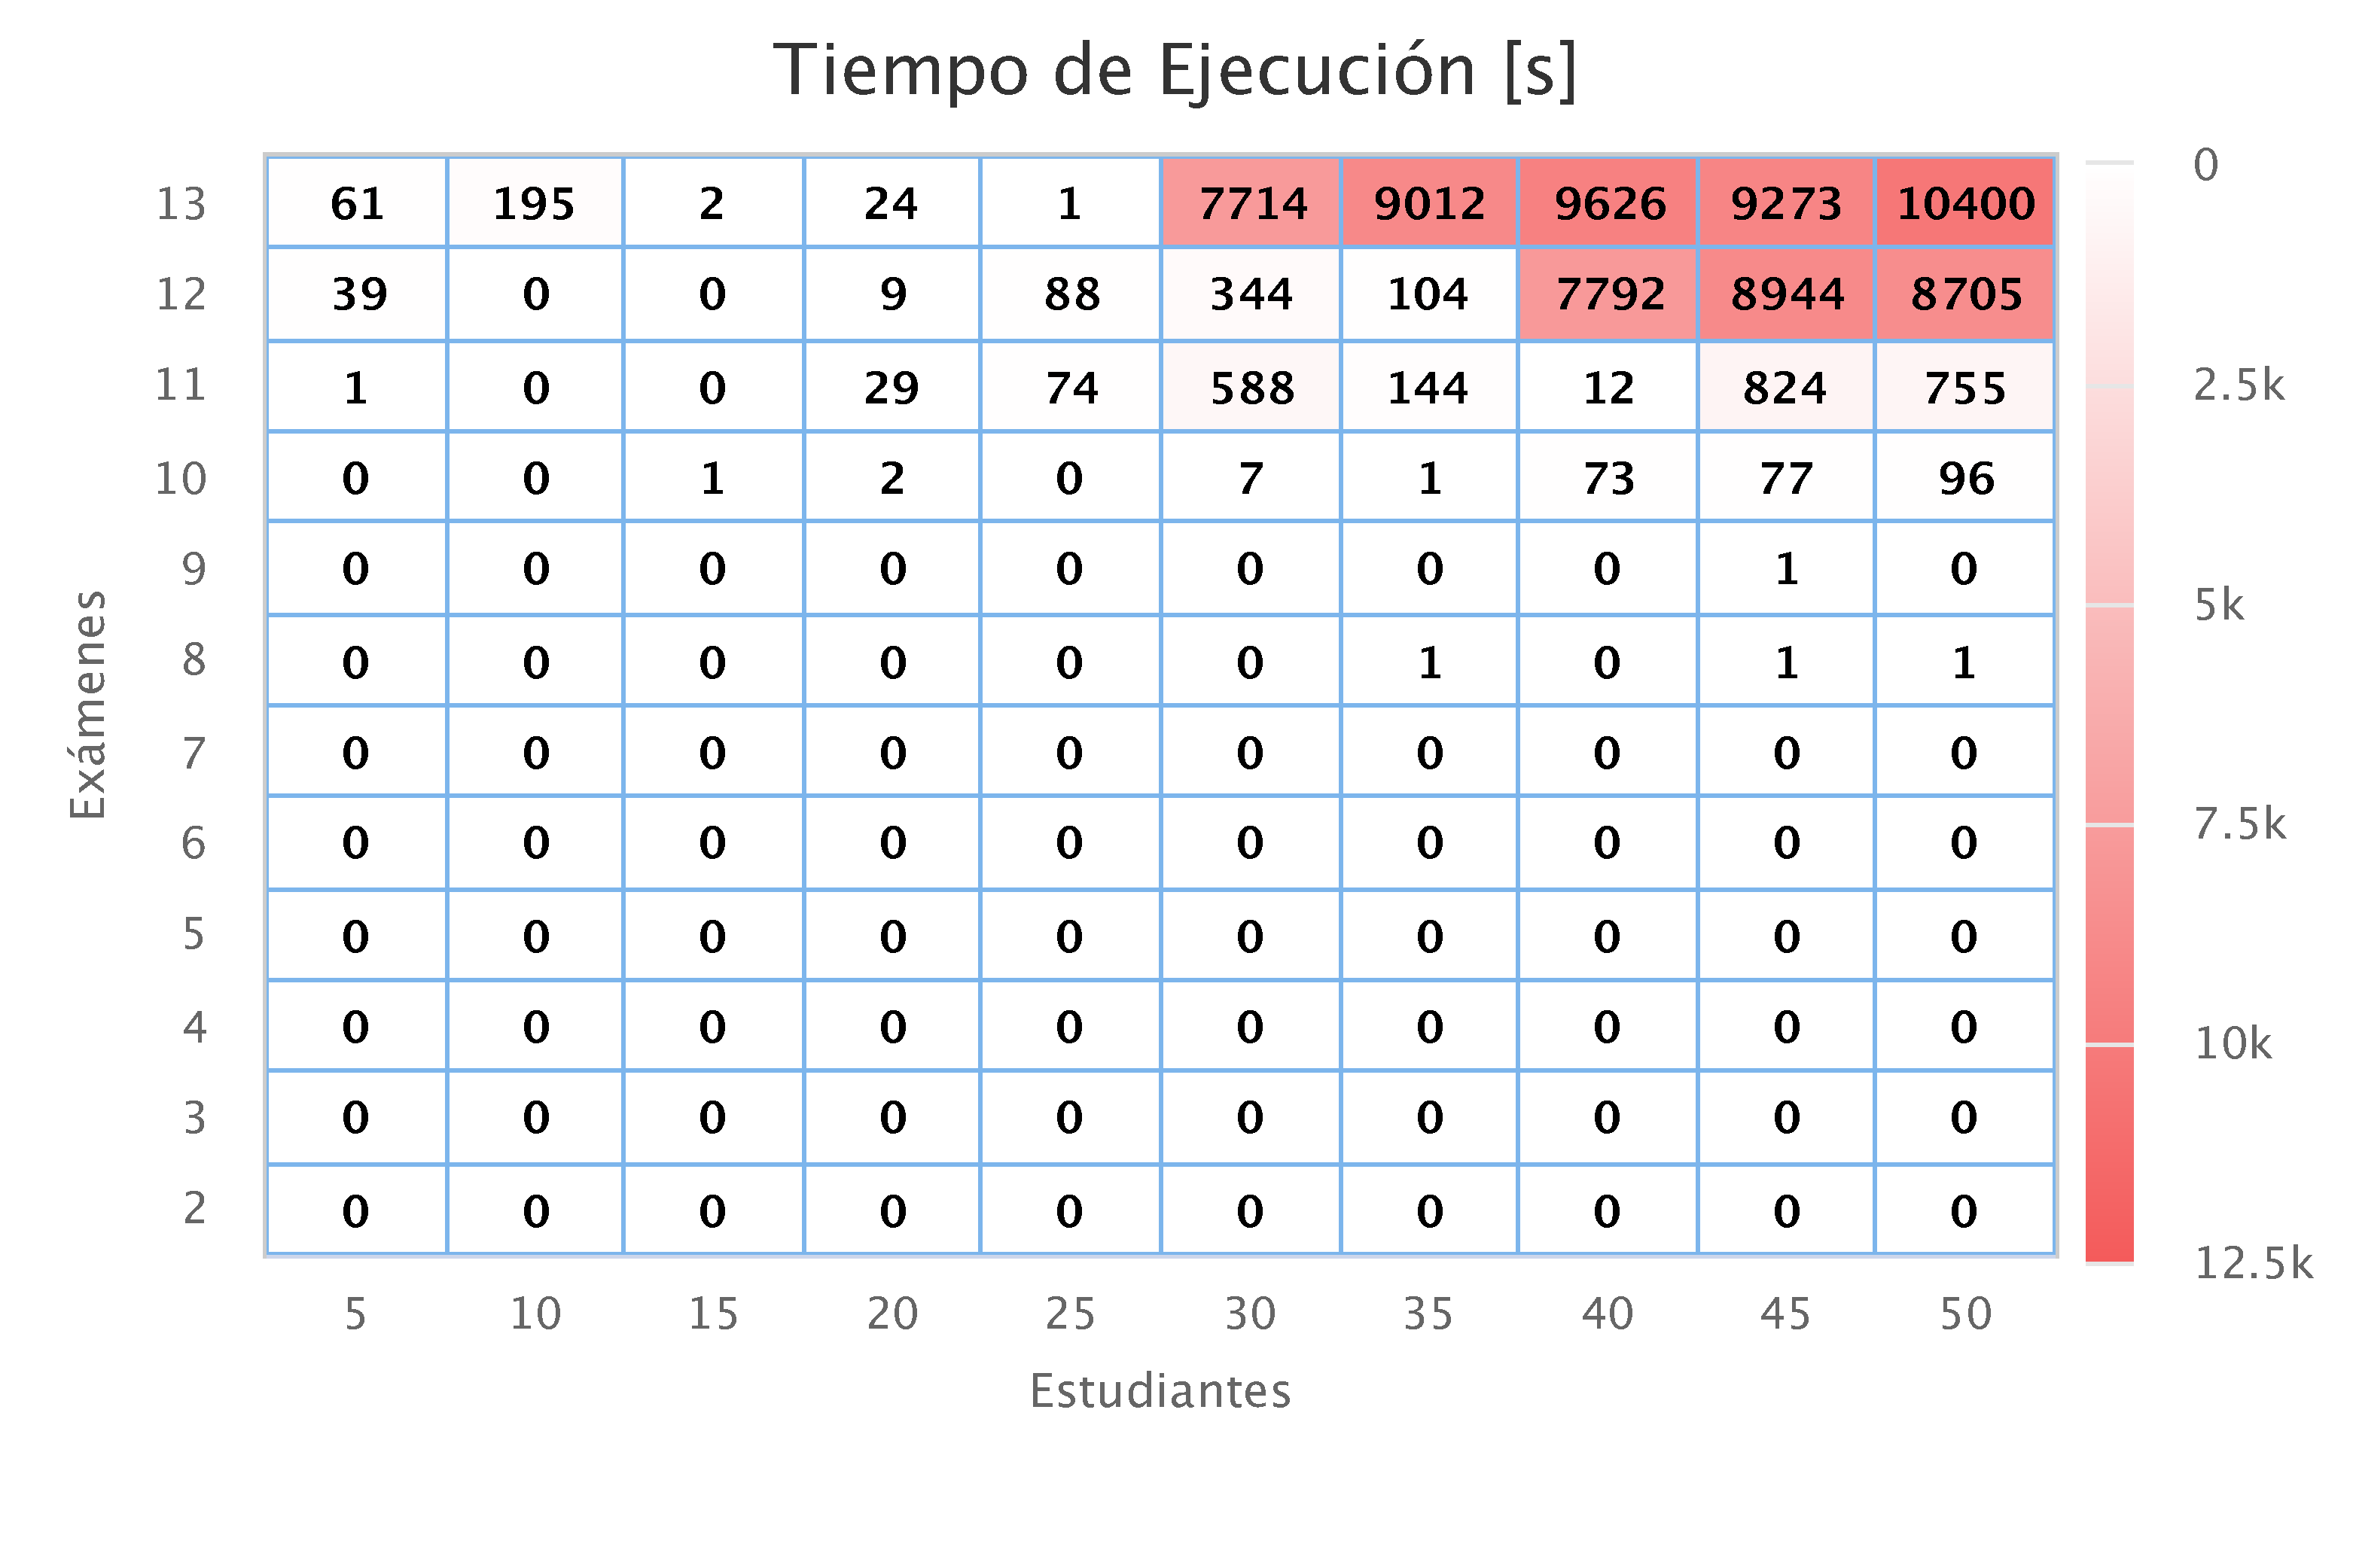
\includegraphics[width=0.7\textwidth]{img/g1.pdf}
\end{center}
\caption{Mapa de calor del tiempo que tardan en resolverse las instancias según la cantidad de exámenes versus estudiantes que éstas tienen.}
\label{fig:g1}
\end{figure}

Se puede apreciar que los tiempos de resolución se alinean con la dificultad de resolver un problema según la cantidad de restricciones, para los casos de la mitad izquierda de la tabla hay muy pocas restricciones y por lo tanto, es muy fácil para el solver encontrar una solución óptima, lo mismo pasa en la esquina inferior derecha del mapa de calor, pues las restricciones son demasiadas y el espacio de búsqueda es muy pequeño. Para las instancias de la esquina superior derecha del mapa de calor hay una cantidad ``media'' de restricciones así como también un espacio de búsqueda enorme, lo que hace que los tiempos aumenten considerablemente.

\begin{figure}[H]
\begin{center}
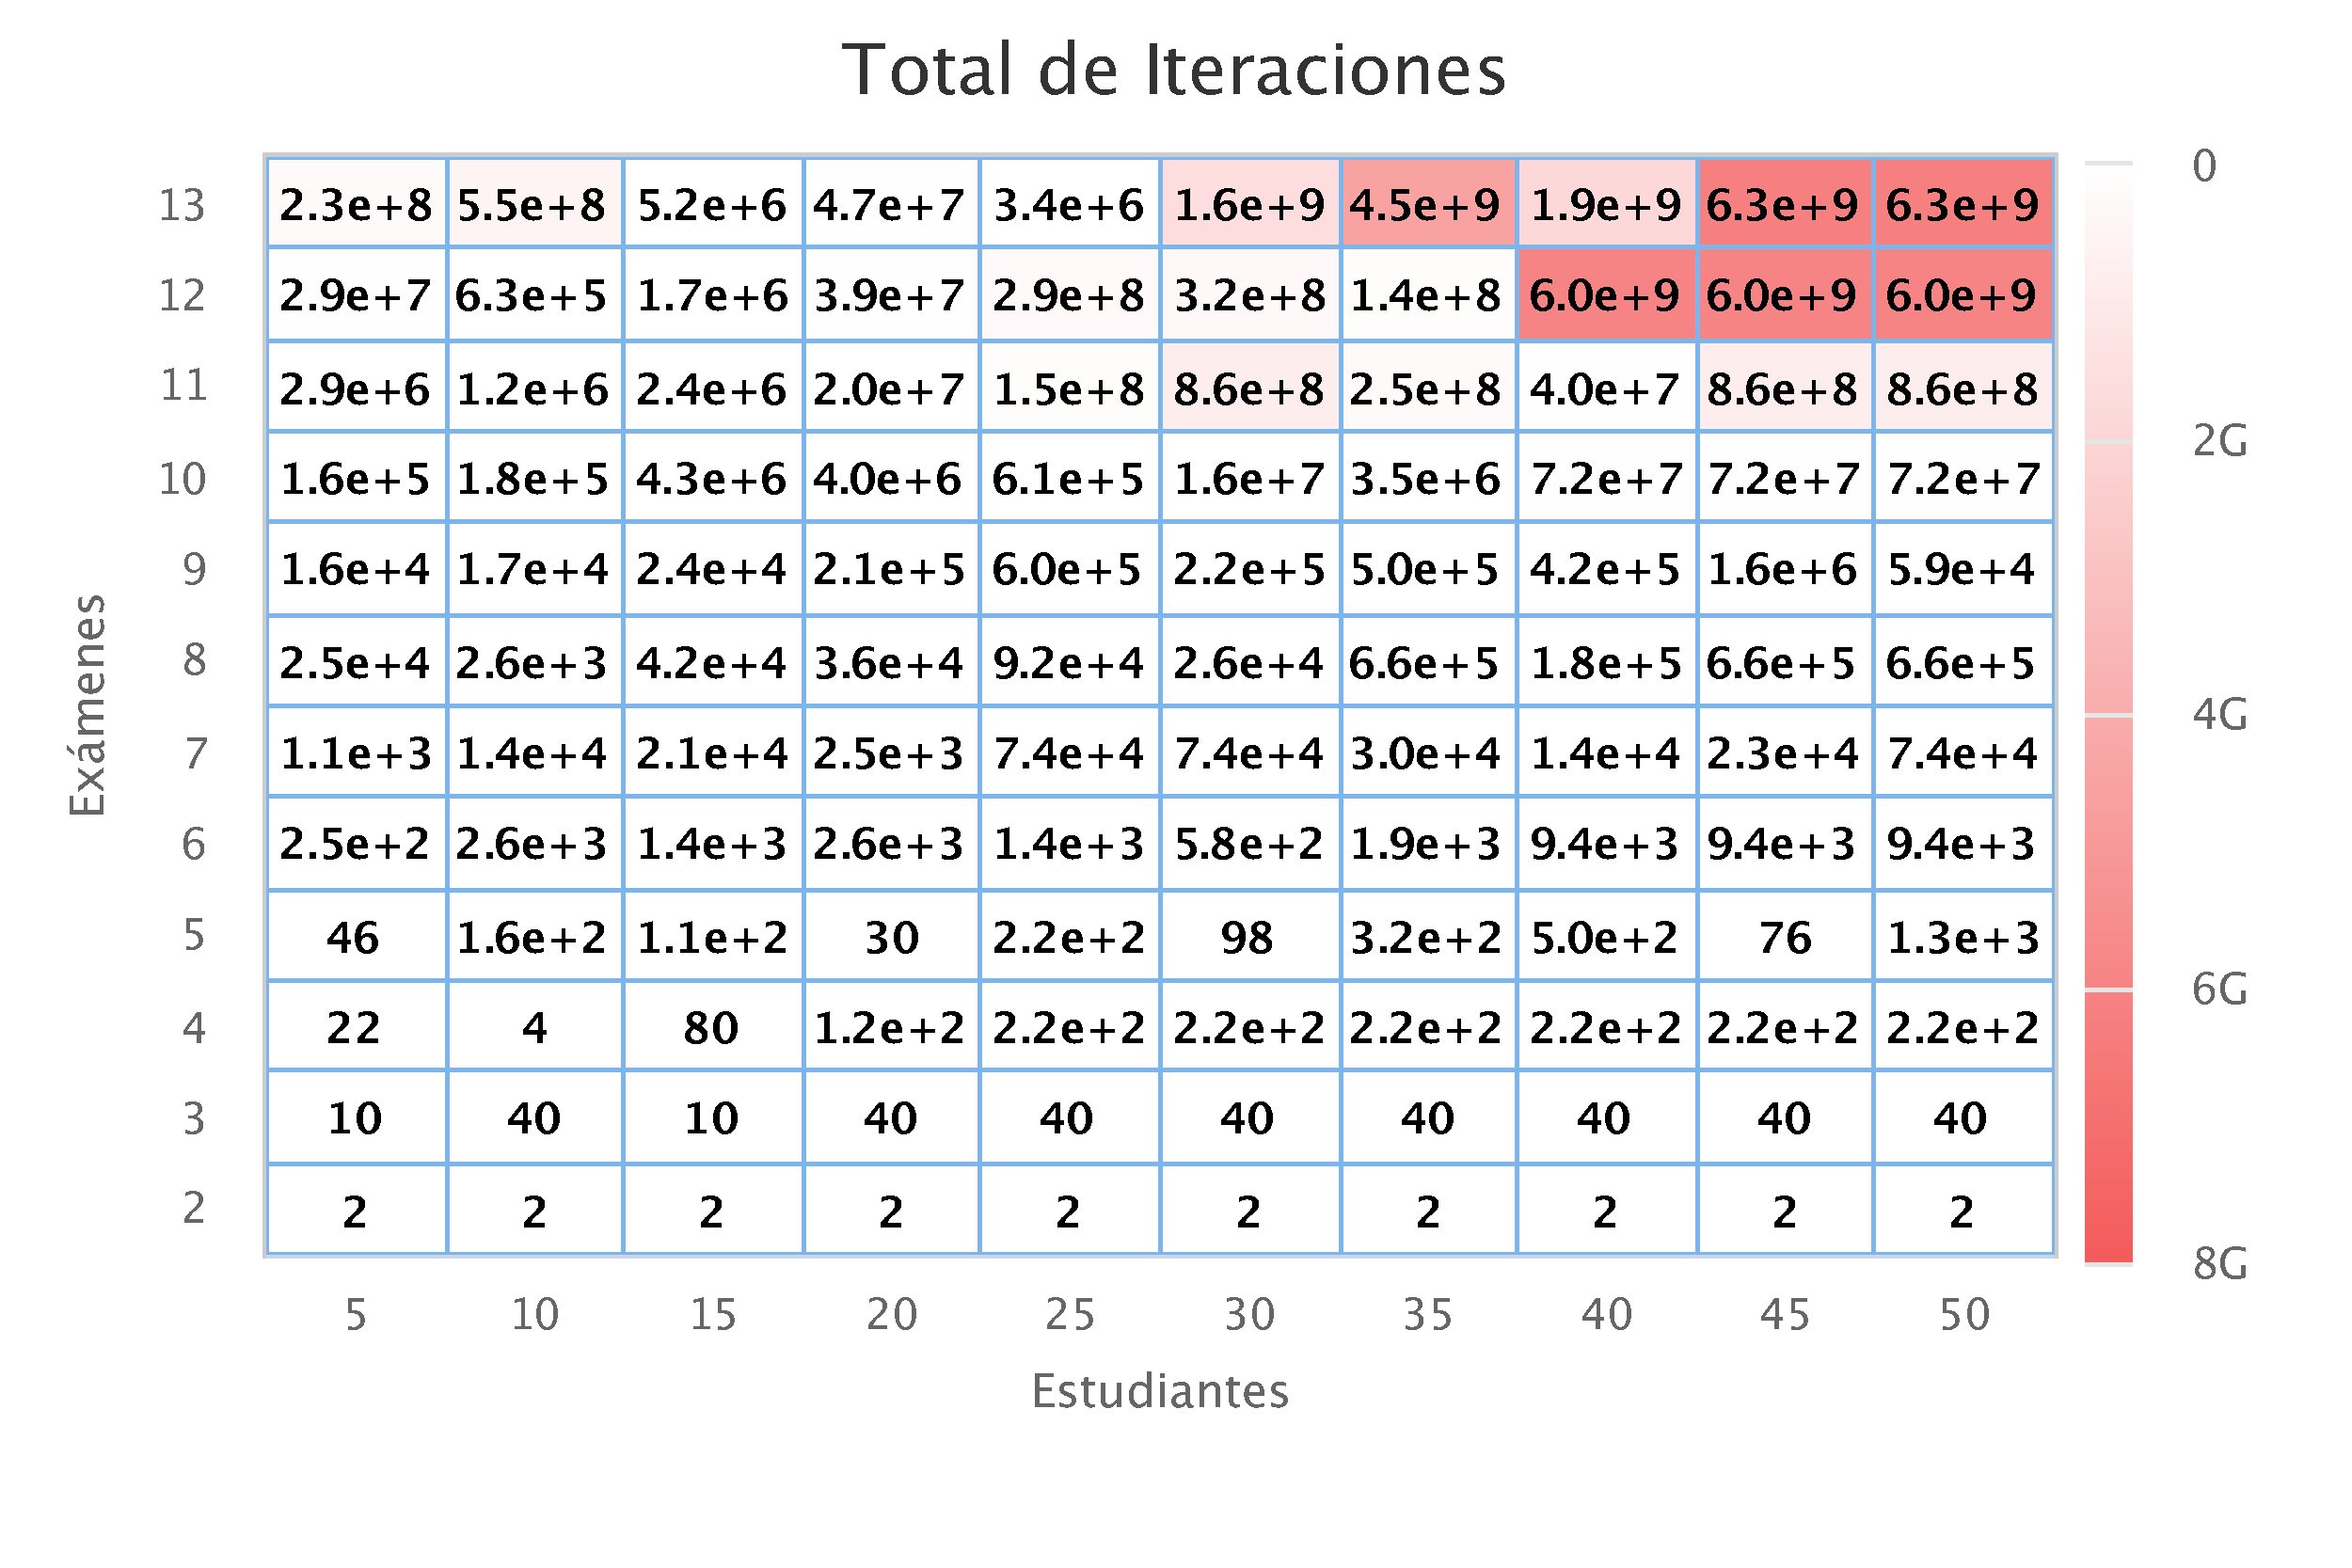
\includegraphics[width=0.7\textwidth]{img/g2.pdf}
\end{center}
\caption{Mapa de calor de las iteraciones realizadas para resolver las instancias según la cantidad de exámenes versus estudiantes que éstas tienen (expresado en notación científica).}
\label{fig:g2}
\end{figure}

En el caso de la cantidad de iteraciones, el análisis es el mismo que el de los tiempos, pues la dificultad de encontrar soluciones se ajusta según el balance de la cantidad de restricciones y por ende, la mayor cantidad de iteraciones se concentra en la esquina superior derecha del mapa de calor. 

\begin{figure}[H]
\begin{center}
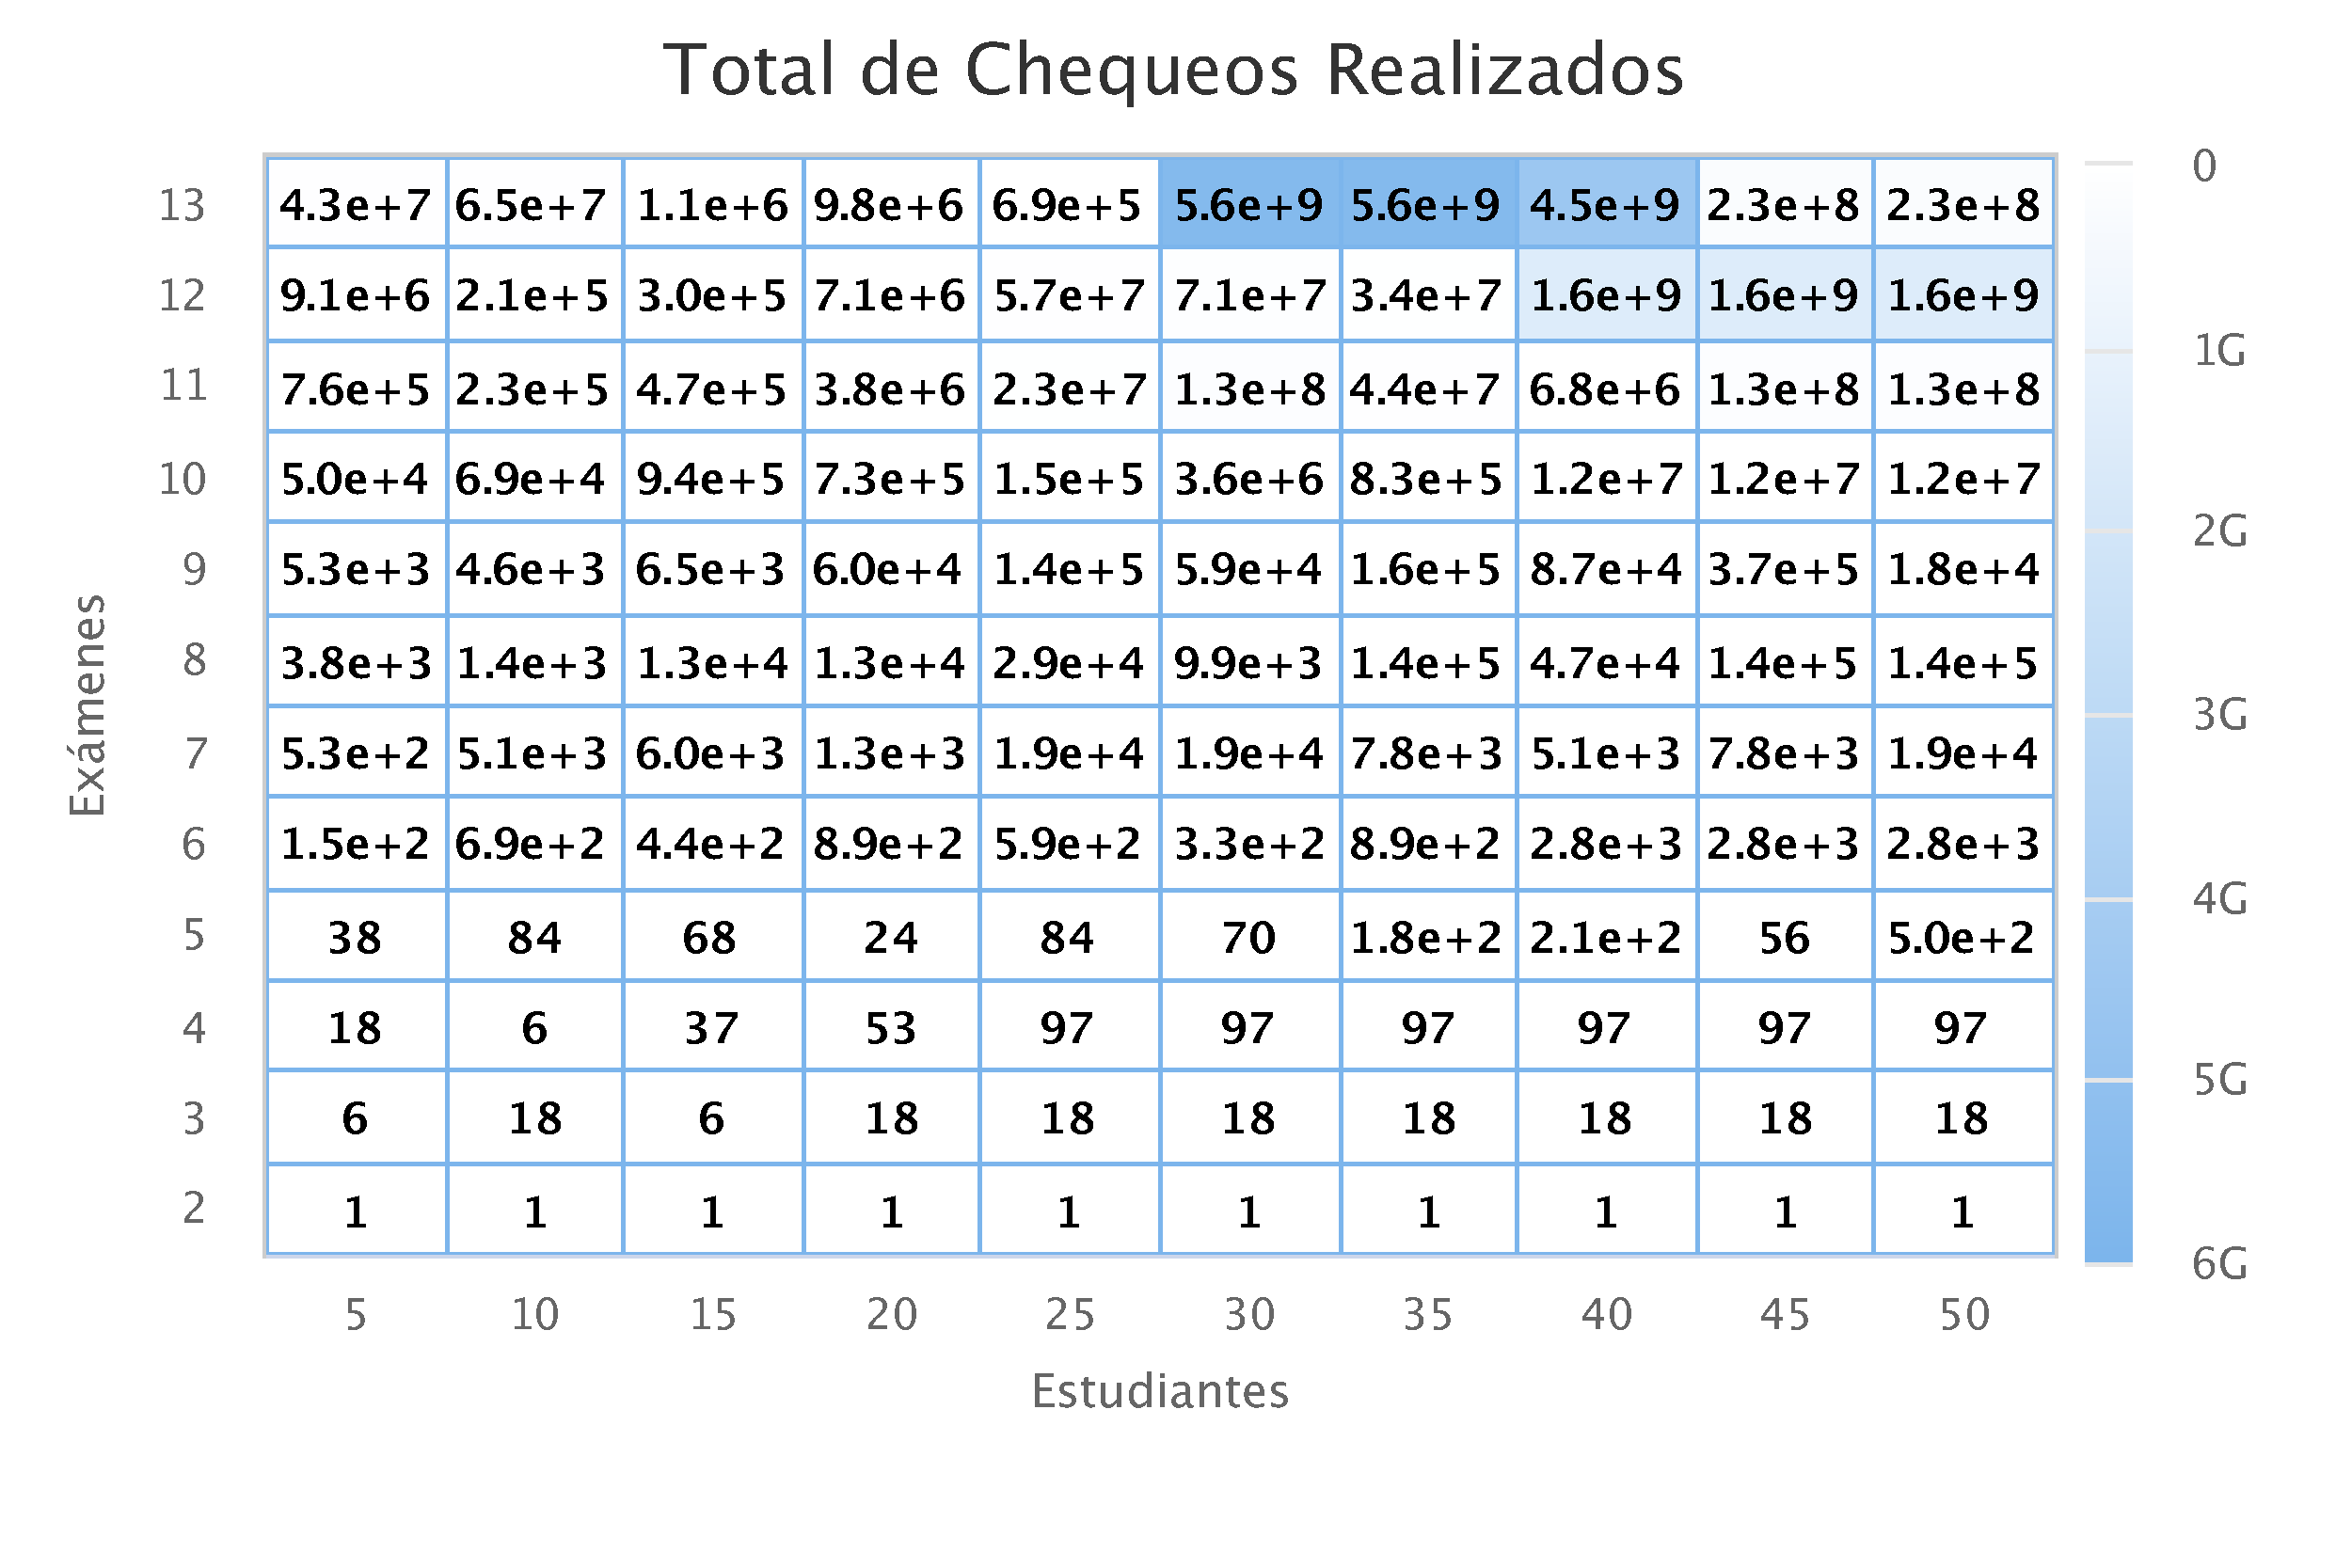
\includegraphics[width=0.7\textwidth]{img/g3.pdf}
\end{center}
\caption{Mapa de calor de los chequeos realizados para resolver las instancias según la cantidad de exámenes versus estudiantes que éstas tienen (expresado en notación científica).}
\label{fig:g3}
\end{figure}

Para los chequeos la situación es distinta, si bien la mayor cantidad de chequeos se concentra cerca de la esquina superior derecha, no es ésta precisamente la instancia de la esquina la que concentra los mayores valores si no las instancias cercanas. Ésto se debe a la efectividad del filtrado que realiza el Forward Checking aplicado en cada asignación de un horario a un examen, pues mientras más restricciones hayan, más probabilidades hay de que el dominio de algún examen (vale decir, sus horarios disponibles) quede vacío y se pueda cortar la rama.

\begin{figure}[H]
\begin{center}
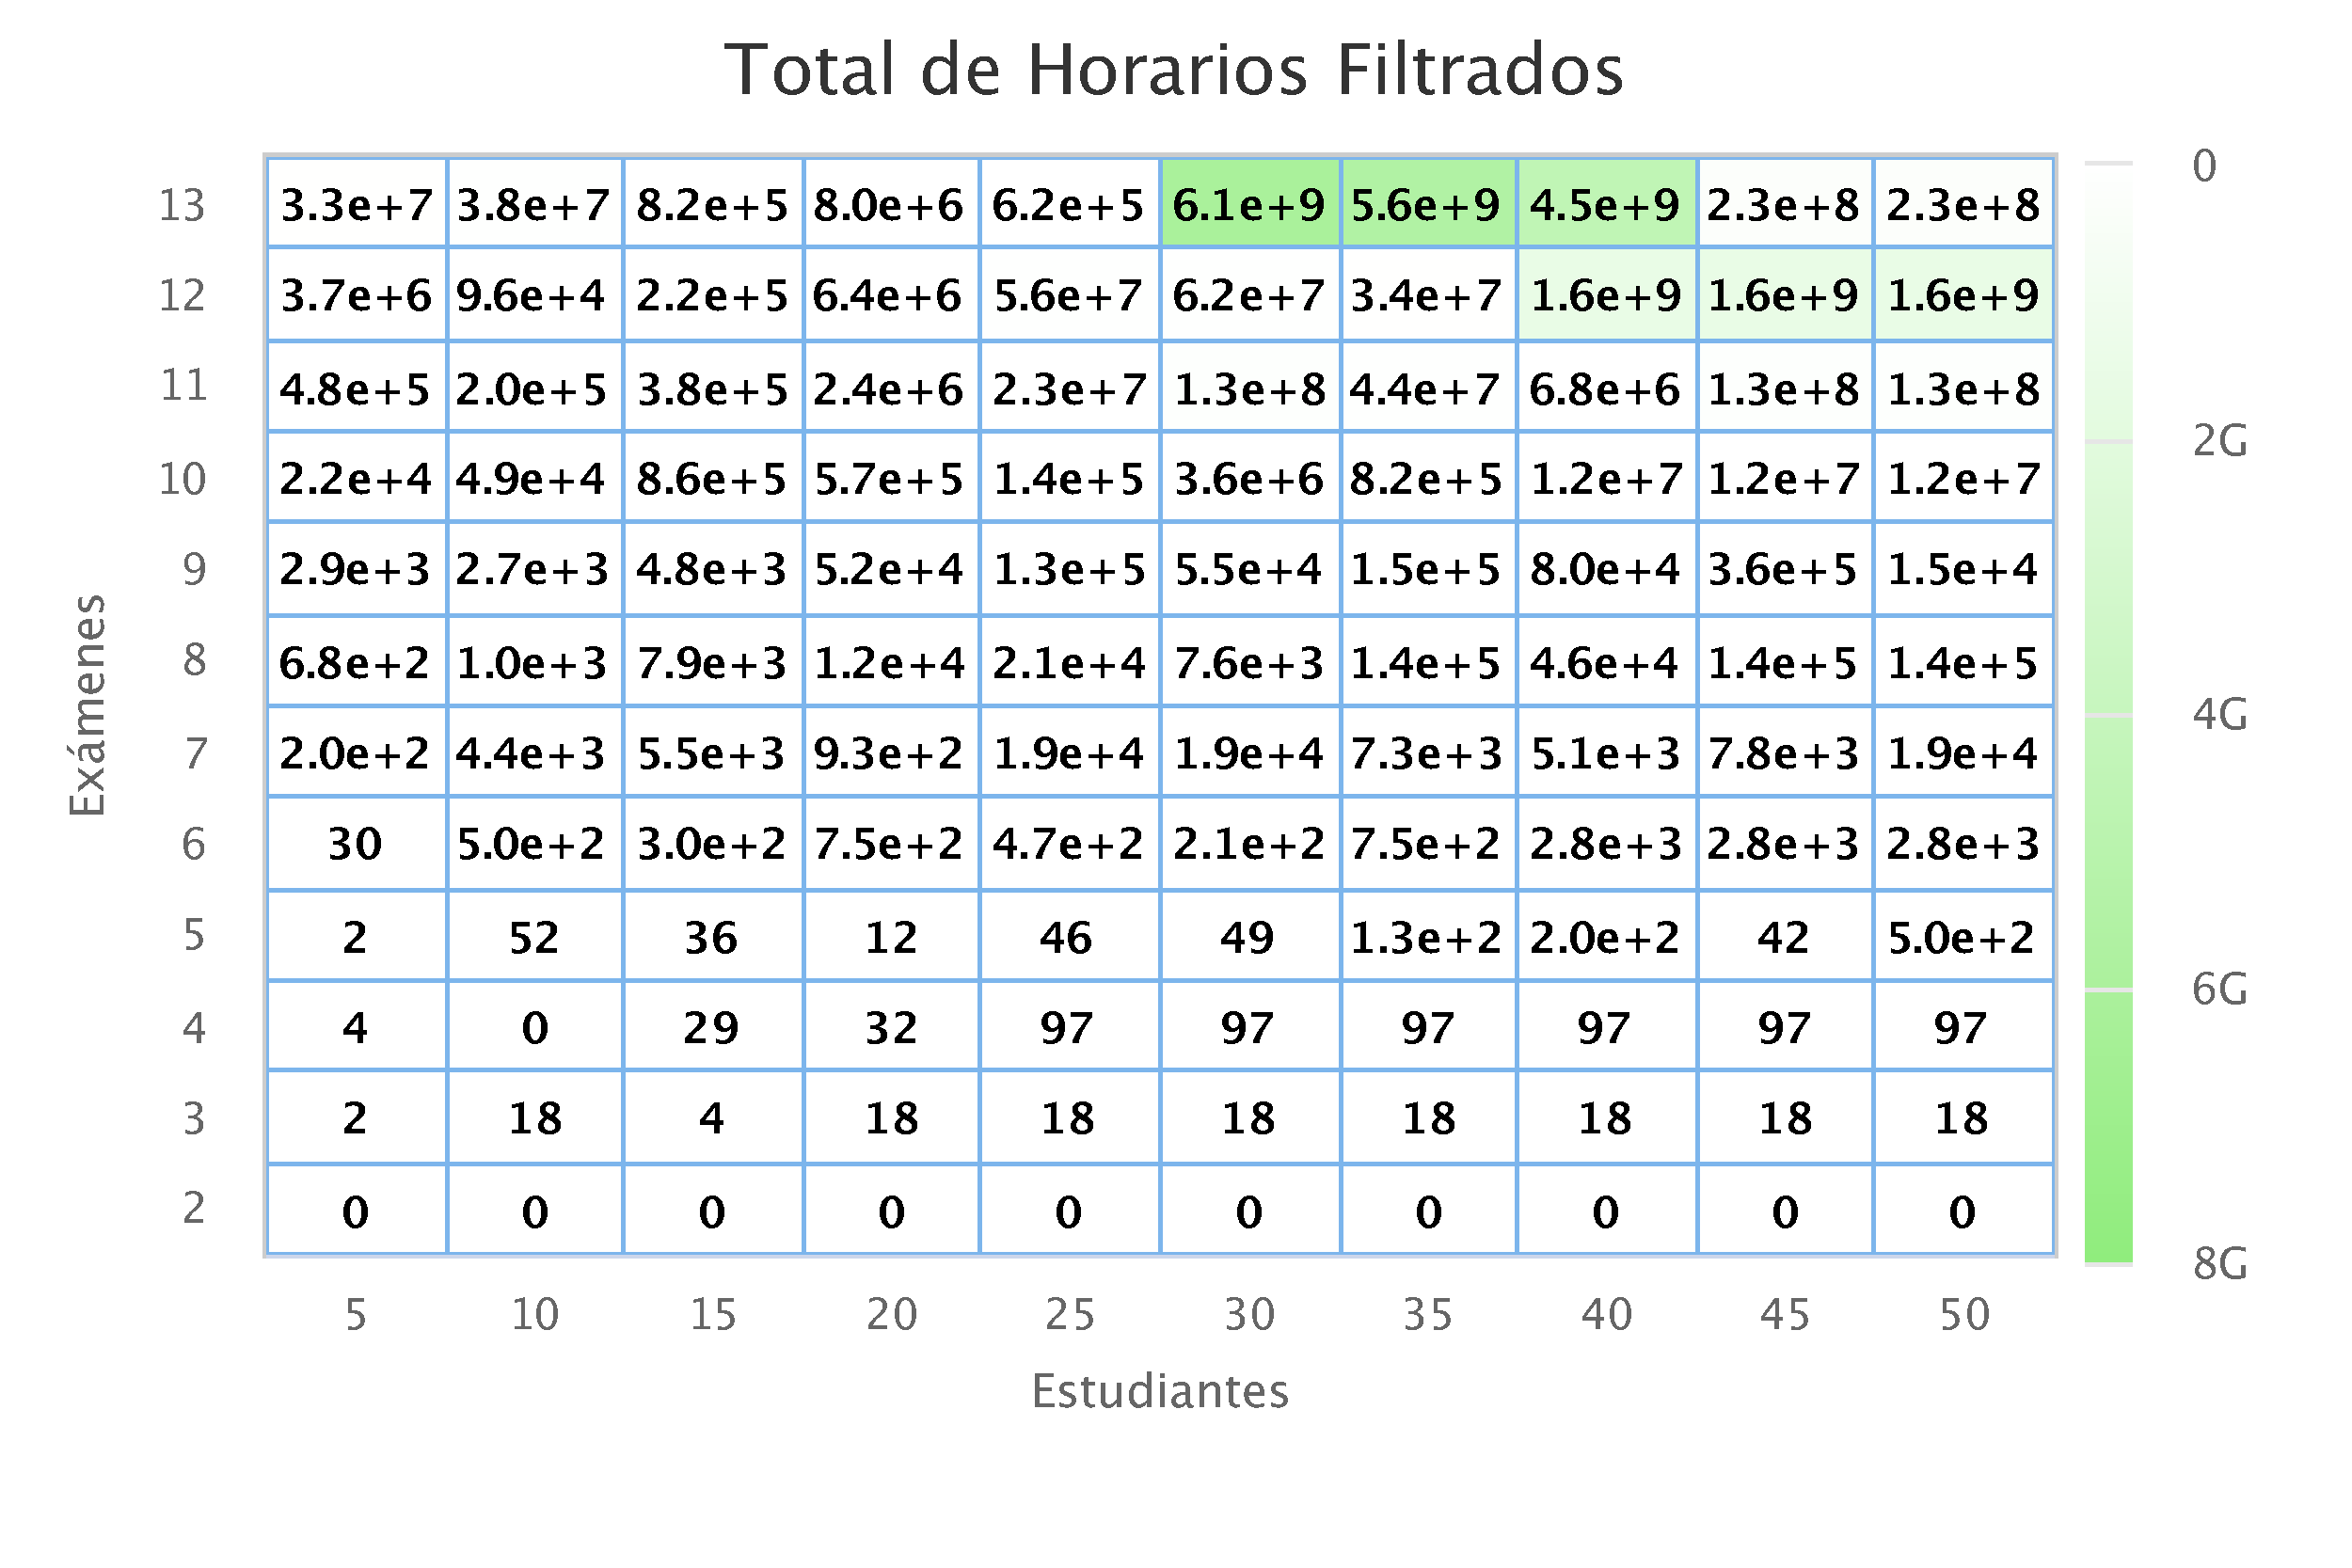
\includegraphics[width=0.7\textwidth]{img/g4.pdf}
\end{center}
\caption{Mapa de calor de los filtros realizados a los horarios disponibles de los exámenes para resolver las instancias según la cantidad de exámenes versus estudiantes que éstas tienen (expresado en notación científica).}
\label{fig:g4}
\end{figure}

En el caso de los horarios filtrados, se asemejan bastante a la cantidad de chequeos realizados, particularmente porque en Forward Checking para filtrar un dominio se debe realizar el chequeo correspondiente, además, para la implementación particular según el \textit{Algoritmo 4} cuando un examen queda sin horarios a asignar, tampoco se siguen filtrando los exámenes posteriores, de hacerlo, se verían números más grandes aquí pero empeoraría el desempeño del algoritmo.

\begin{figure}[H]
\begin{center}
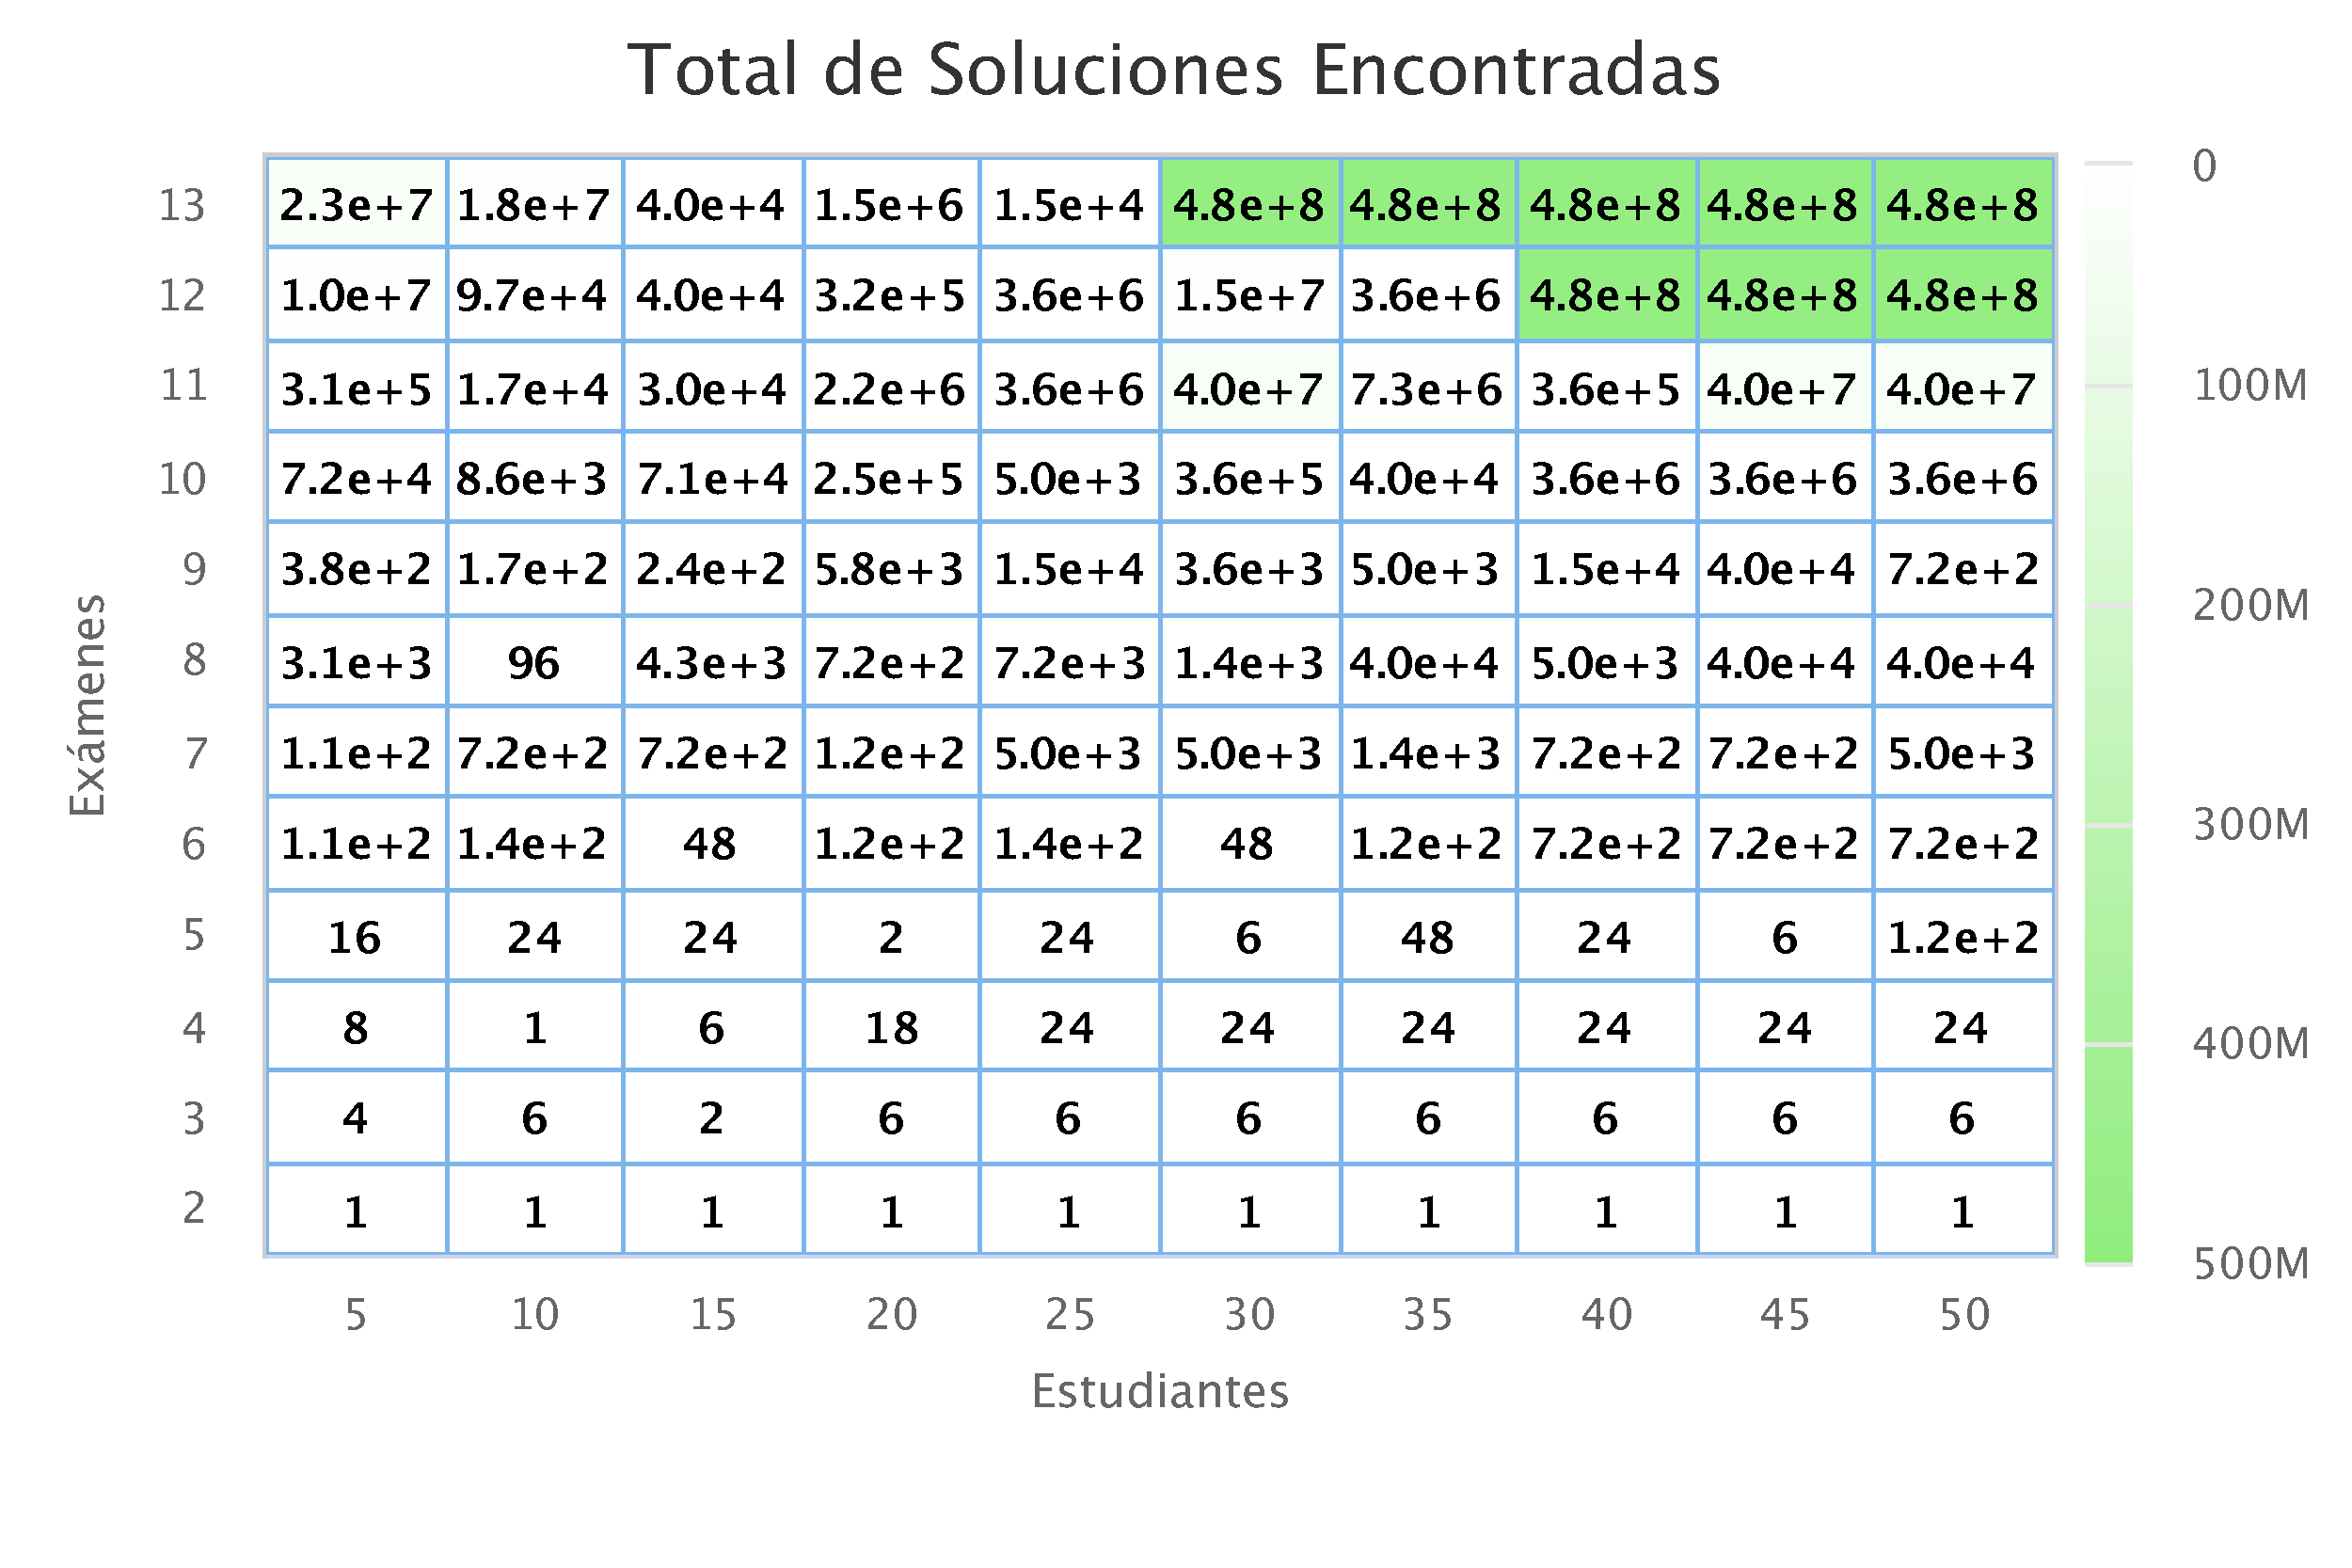
\includegraphics[width=0.7\textwidth]{img/g5.pdf}
\end{center}
\caption{Mapa de calor las soluciones encontradas a la hora de resolver las instancias según la cantidad de exámenes versus estudiantes que éstas tienen (expresado en notación científica).}
\label{fig:g5}
\end{figure}

En el caso de las soluciones encontradas, se puede apreciar que mientras más grande es el espacio de búsqueda, más soluciones pueden encontrarse, ésto debido particularmente al hecho de que existe todo un espacio de búsqueda factible de $E!$ equivalente a las combinaciones de asignar 1 horario distinto a cada examen, por lo que mientras más exámenes, más soluciones factibles hay.

\begin{figure}[H]
\begin{center}
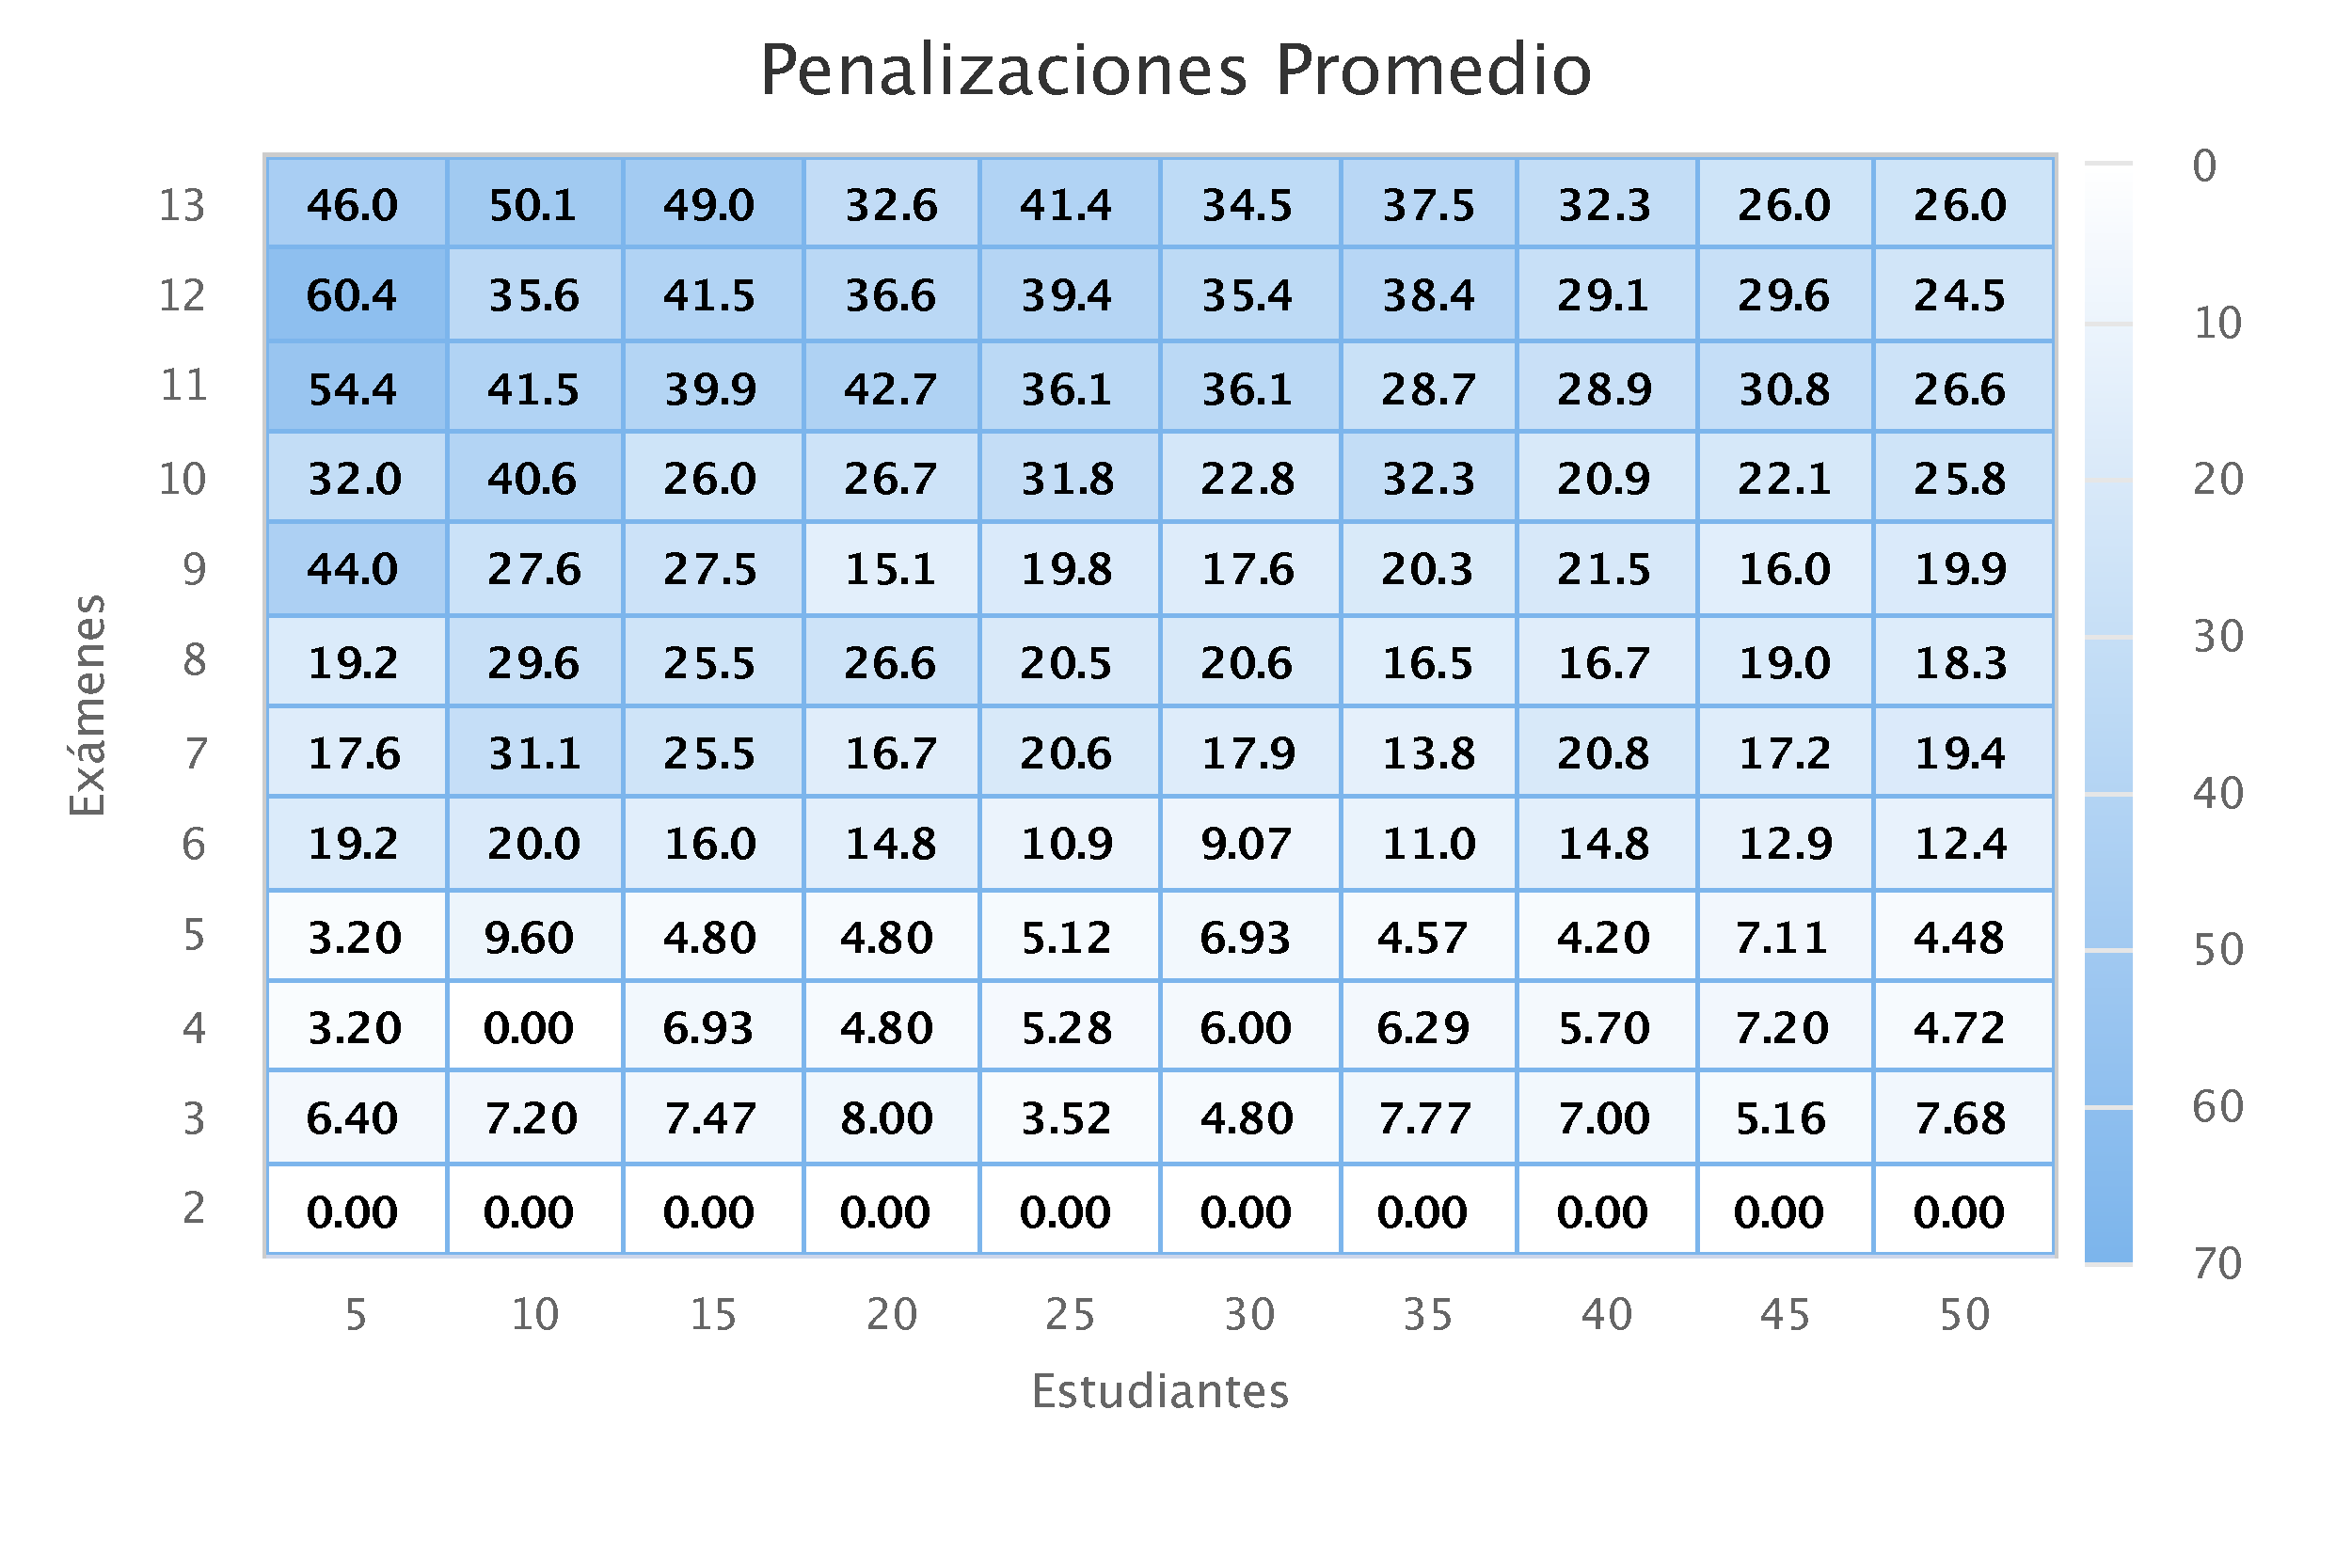
\includegraphics[width=0.7\textwidth]{img/g6.pdf}
\end{center}
\caption{Mapa de calor la penalización promedio obtenida en cada instancia resuelta según la cantidad de exámenes versus estudiantes que éstas tienen.}
\label{fig:g6}
\end{figure}

En el caso de las penalizaciones es interesante notar que para casos donde cada estudiante sólo tiene 1 examen asignado no hay penalización, mientras que para casos donde la cantidad de estudiantes es poca pero la de exámenes mucha, la penalización de la solución óptima aumenta bastante, concentrándose los valores más altos en la esquina superior izquierda del mapa de calor

\begin{figure}[H]
\begin{center}
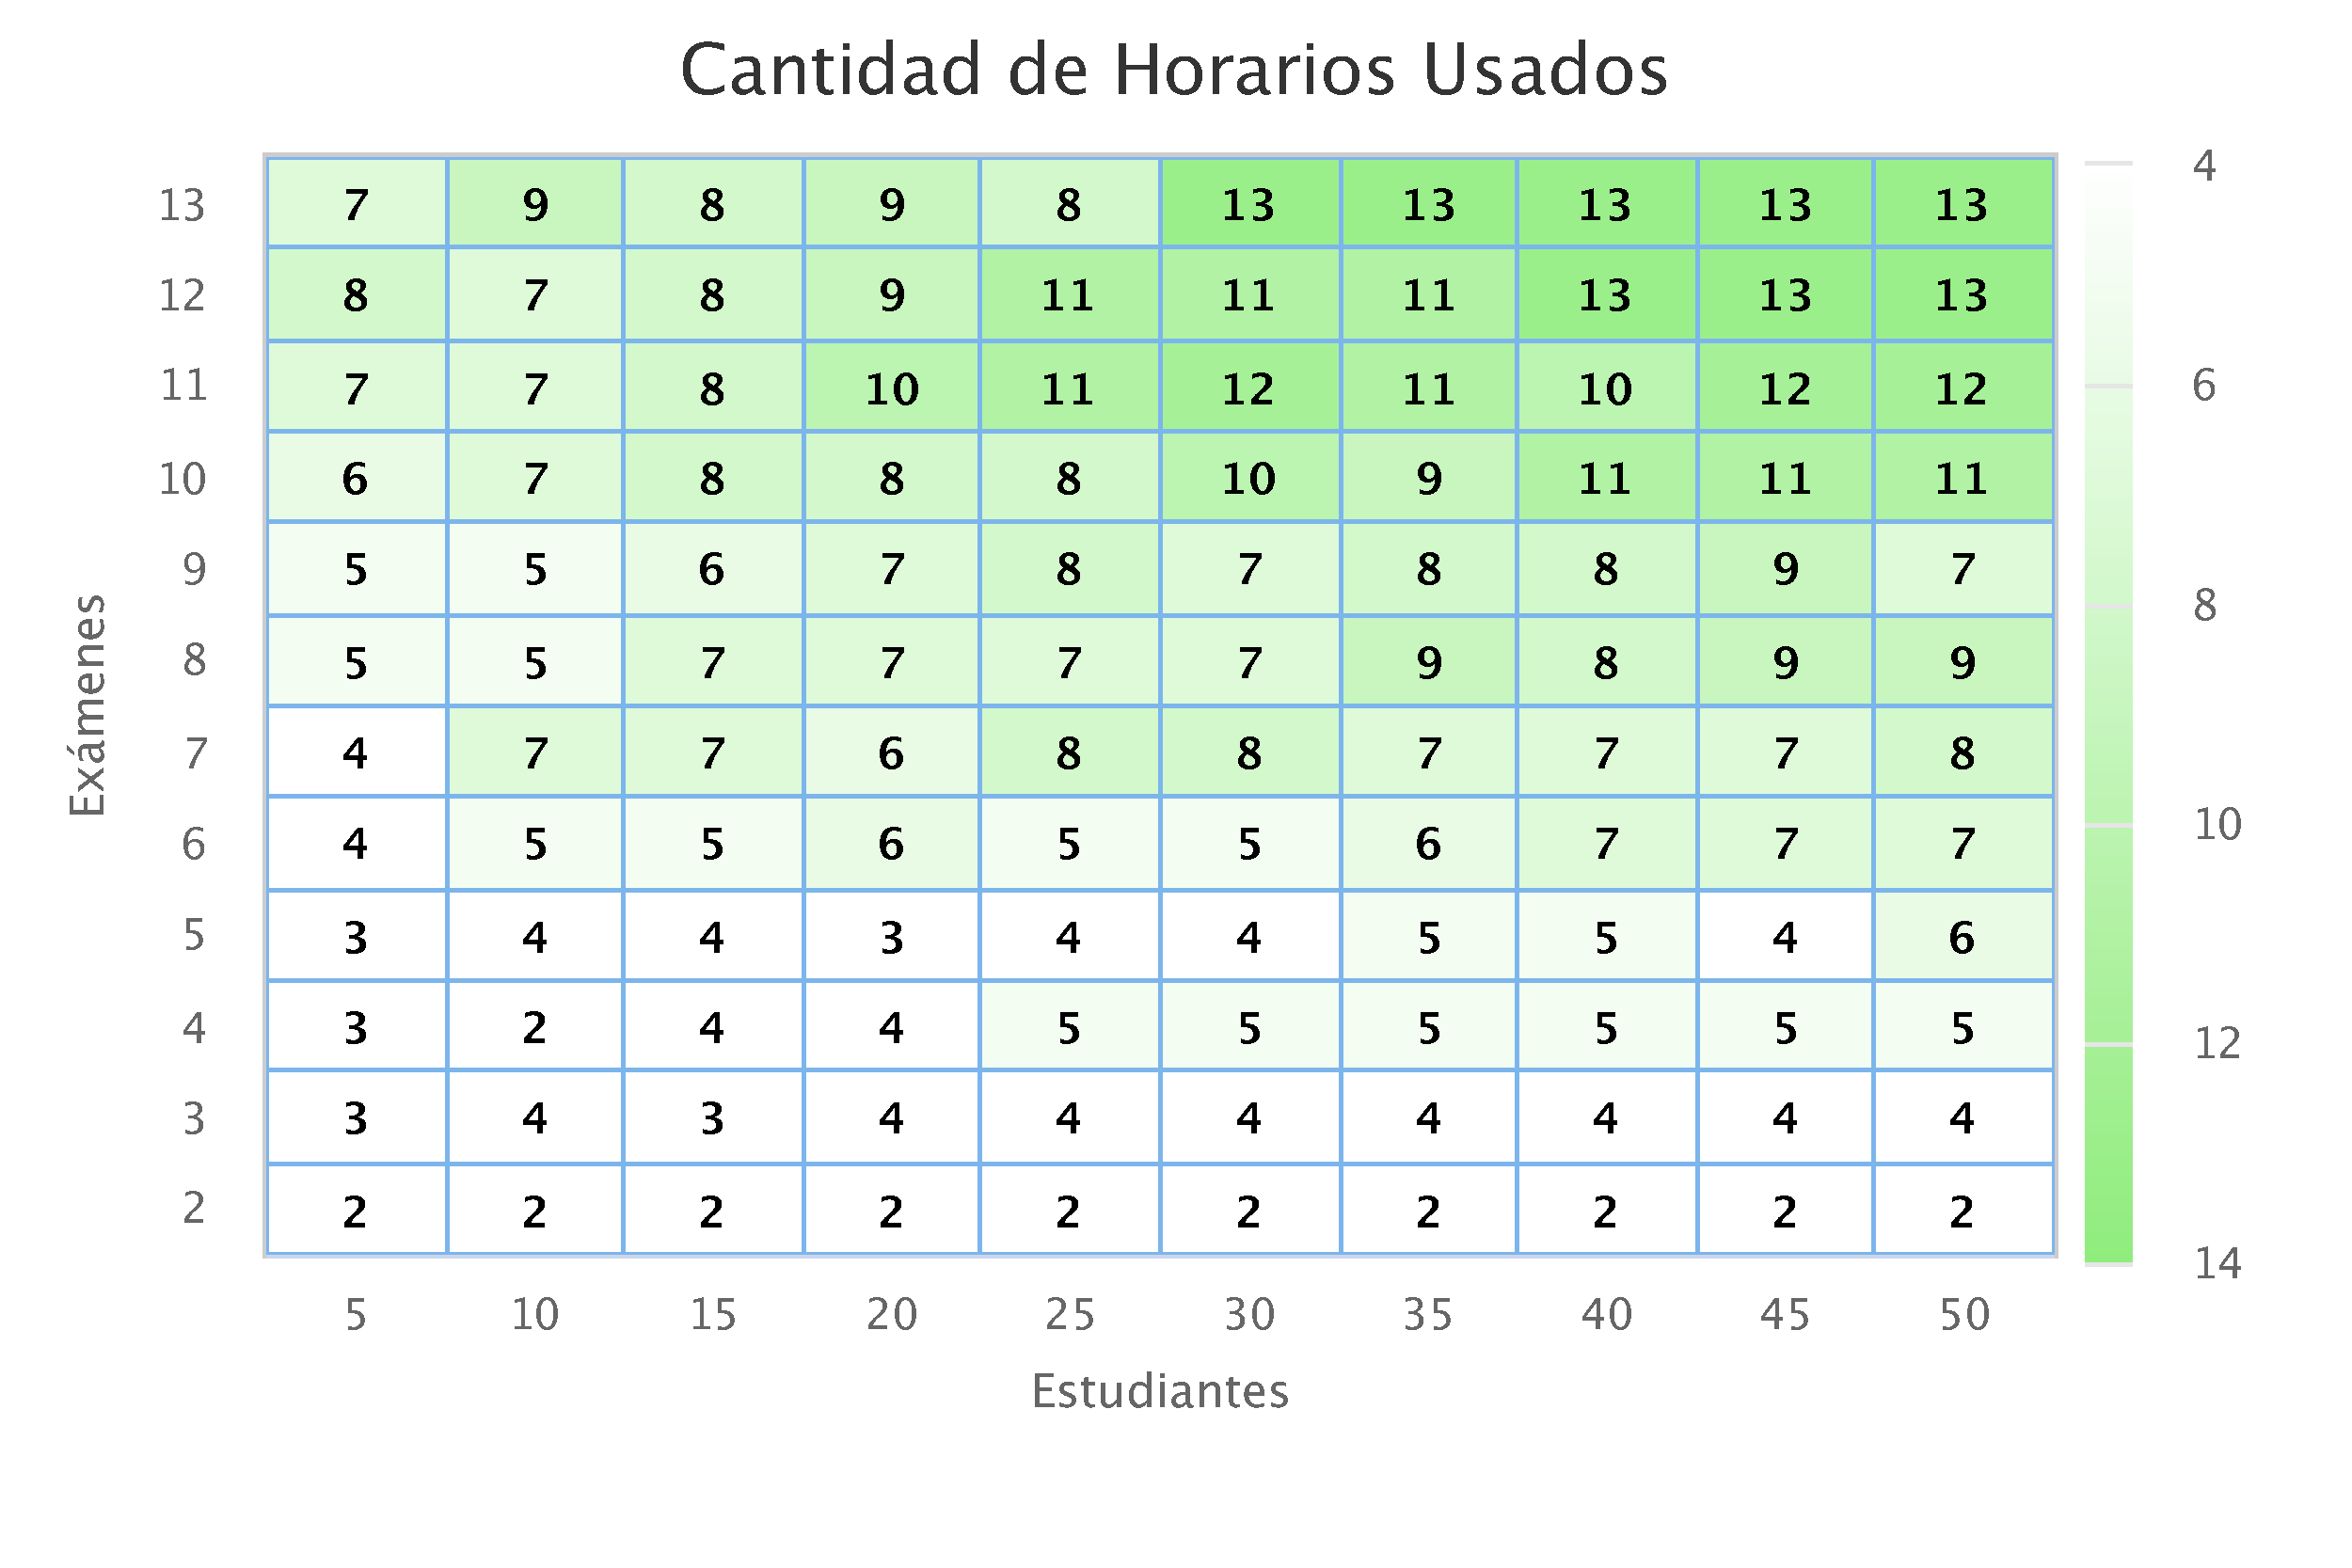
\includegraphics[width=0.7\textwidth]{img/g7.pdf}
\end{center}
\caption{Mapa de calor de la cantidad de horarios obtenida en cada instancia resuelta según la cantidad de exámenes versus estudiantes que éstas tienen (expresado en notación científica).}
\label{fig:g6}
\end{figure}

Finalmente, se puede apreciar que mientras más estudiantes y exámenes estén involucrados en la instancia, más horarios se requerirán para poder realizar una calendarización óptima.

\section{Conclusiones} \label{conclusiones}

El ETP es un problema arduamente estudiado gracias a su importancia e impacto en las instituciones educacionales, los avances en su resolución se traducen en mejores condiciones para los estudiantes a la hora de rendir sus exámenes y mejores planificaciones para la institución, no obstante, las distintas realidades de éstas hacen que los investigadores se concentren en resolver distintas variantes generando así soluciones no aplicables a todas las instituciones. Pese a esto, las distintas técnicas implementadas han permitido ahondar en cómo cada una se puede ajustar para obtener mejores resultados en la institución particular donde el autor se centra, pero al mismo tiempo no suelen ser tan buenas cuando se aplican de manera general. Esto se visualiza en como los parámetros de de la mayoría de técnicas se pueden ajustar para ser excelentes en ciertos casos o en como las técnicas exactas funcionan bien para instituciones que requieren calendarizar pocos exámenes, sin lograr ser las mejores a la hora de hacer benchmarks estandarizados, ante este escenario, las técnicas basadas en híbridos con hyperheurísticas se posicionan como las técnicas más prometedoras para atacar este problema. Forward Checking en cambio se posiciona como una buena alternativa de resolución al problema para casos con instancias muy pequeñas, particularmente con pocos exámenes y una cantidad no considerable de estudiantes, no obstante, para instancias más grandes asociadas a la realidad de las universidades, esta técnica no permite obtener buenos resultados en tiempos razonables. Por otro lado, Forward Checking permite estudiar el comportamiento de ciertos aspectos de las instancias cuando éstas son pequeñas, basado en los resultados obtenidos en la sección anterior se obtienen conclusiones interesantes respecto de como crece la cantidad de horarios necesarios para generar calendarizaciones óptimas en base a la cantidad de exámenes y estudiantes, lo mismo aplica para el aumento de la penalización promedio a medida que la cantidad de estudiantes disminuye, todos estos análisis y otras conclusiones son posibles gracias a la aplicación de Forward Checking y permiten establecer criterios para el desarrollo de nuevas soluciones basadas en heurísticas que se ajusten mejor a la obtención de soluciones rápidas y efectivas para el problema. A futuro se plantea ahondar en la investigación basada en técnicas híbridas con hyperheurísticas que se ejecuten en paralelo utilizando CUDA \cite{cuda}, para así estudiar espacios de soluciones en paralelo con el fin de acelerar el proceso.


\section*{Bibliografía}
\bibliographystyle{plain}
\bibliography{Referencias}

\section*{Anexo A}

Detalle de las instancias usadas en la experimentación junto con sus resultados, la orientación de la tabla se cambió para que quepa en el documento, lo mismo con nombres de las columnas se ajustaron según la siguiente nomenclatura:

\begin{itemize}
	\item \textbf{E}: Exámenes
	\item \textbf{S}: Estudiantes
	\item \textbf{C}: Total de conflictos
	\item \textbf{A}: Total de exámenes asignados.
	\item \textbf{Amax}: Cantidad máxima de exámenes asignados a un estudiante
	\item \textbf{T}: Horarios usados para resolver la instancia
\end{itemize}

Cabe destacar que algunas instancias de 14 y 15 exámenes no aparecen porque no pudieron ser resueltas durante el tiempo de experimentación, por lo mismo se omitieron en la tabla y en los resultados.

\begin{landscape}
\begin{longtable}{|c|c|c|c|c|c|c|c|c|c|c|c|c|c|}

Instancia & E & S & C & A & Amax & T & Penalización & Iteraciones & Chequeos & Filtros & Soluciones & Mejoras a la Solución & Tiempo \\
\hline
E2S5 & 2 & 5 & 0 & 5 & 1 & 2 & 0.0 & 2 & 1 & 0 & 1 & 1 & 0.0001 \\
E2S10 & 2 & 10 & 0 & 10 & 1 & 2 & 0.0 & 2 & 1 & 0 & 1 & 1 & 0.0001 \\
E2S15 & 2 & 15 & 0 & 15 & 1 & 2 & 0.0 & 2 & 1 & 0 & 1 & 1 & 0.0001 \\
E2S20 & 2 & 20 & 0 & 20 & 1 & 2 & 0.0 & 2 & 1 & 0 & 1 & 1 & 0.0001 \\
E2S25 & 2 & 25 & 0 & 25 & 1 & 2 & 0.0 & 2 & 1 & 0 & 1 & 1 & 0.0001 \\
E2S30 & 2 & 30 & 0 & 30 & 1 & 2 & 0.0 & 2 & 1 & 0 & 1 & 1 & 0.0001 \\
E2S35 & 2 & 35 & 0 & 35 & 1 & 2 & 0.0 & 2 & 1 & 0 & 1 & 1 & 0.0001 \\
E2S40 & 2 & 40 & 0 & 40 & 1 & 2 & 0.0 & 2 & 1 & 0 & 1 & 1 & 0.0001 \\
E2S45 & 2 & 45 & 0 & 45 & 1 & 2 & 0.0 & 2 & 1 & 0 & 1 & 1 & 0.0001 \\
E2S50 & 2 & 50 & 0 & 50 & 1 & 2 & 0.0 & 2 & 1 & 0 & 1 & 1 & 0.0001 \\
E3S5 & 3 & 5 & 1 & 7 & 2 & 3 & 6.4 & 10 & 6 & 2 & 4 & 1 & 0.0001 \\
E3S10 & 3 & 10 & 3 & 16 & 2 & 4 & 7.2 & 40 & 18 & 18 & 6 & 1 & 0.0001 \\
E3S15 & 3 & 15 & 2 & 22 & 2 & 3 & 7.4667 & 10 & 6 & 4 & 2 & 1 & 0.0122 \\
E3S20 & 3 & 20 & 3 & 31 & 2 & 4 & 8.0 & 40 & 18 & 18 & 6 & 1 & 0.0001 \\
E3S25 & 3 & 25 & 3 & 32 & 2 & 4 & 3.52 & 40 & 18 & 18 & 6 & 1 & 0.0001 \\
E3S30 & 3 & 30 & 3 & 40 & 2 & 4 & 4.8 & 40 & 18 & 18 & 6 & 1 & 0.0001 \\
E3S35 & 3 & 35 & 3 & 54 & 2 & 4 & 7.7714 & 40 & 18 & 18 & 6 & 1 & 0.0002 \\
E3S40 & 3 & 40 & 3 & 59 & 2 & 4 & 7.0 & 40 & 18 & 18 & 6 & 1 & 0.0001 \\
E3S45 & 3 & 45 & 3 & 62 & 2 & 4 & 5.1556 & 40 & 18 & 18 & 6 & 1 & 0.0002 \\
E3S50 & 3 & 50 & 3 & 78 & 2 & 4 & 7.68 & 40 & 18 & 18 & 6 & 1 & 0.0002 \\
E4S5 & 4 & 5 & 1 & 6 & 2 & 3 & 3.2 & 22 & 18 & 4 & 8 & 1 & 0.0001 \\
E4S10 & 4 & 10 & 0 & 10 & 1 & 2 & 0.0 & 4 & 6 & 0 & 1 & 1 & 0.0001 \\
E4S15 & 4 & 15 & 5 & 22 & 2 & 4 & 6.9333 & 80 & 37 & 29 & 6 & 1 & 0.0001 \\
E4S20 & 4 & 20 & 3 & 27 & 2 & 4 & 4.8 & 115 & 53 & 32 & 18 & 1 & 0.0002 \\
E4S25 & 4 & 25 & 6 & 39 & 2 & 5 & 5.28 & 222 & 97 & 97 & 24 & 1 & 0.0003 \\
E4S30 & 4 & 30 & 6 & 47 & 2 & 5 & 6.0 & 222 & 97 & 97 & 24 & 1 & 0.0003 \\
E4S35 & 4 & 35 & 6 & 53 & 2 & 5 & 6.2857 & 222 & 97 & 97 & 24 & 1 & 0.0003 \\
E4S40 & 4 & 40 & 6 & 58 & 2 & 5 & 5.7 & 222 & 97 & 97 & 24 & 1 & 0.0003 \\
E4S45 & 4 & 45 & 6 & 69 & 2 & 5 & 7.2 & 222 & 97 & 97 & 24 & 1 & 0.0003 \\
E4S50 & 4 & 50 & 6 & 72 & 2 & 5 & 4.72 & 222 & 97 & 97 & 24 & 1 & 0.0003 \\
E5S5 & 5 & 5 & 1 & 6 & 2 & 3 & 3.2 & 46 & 38 & 2 & 16 & 1 & 0.0001 \\
E5S10 & 5 & 10 & 5 & 17 & 2 & 4 & 9.6 & 156 & 84 & 52 & 24 & 1 & 0.0002 \\
E5S15 & 5 & 15 & 5 & 20 & 2 & 4 & 4.8 & 112 & 68 & 36 & 24 & 1 & 0.0002 \\
E5S20 & 5 & 20 & 5 & 26 & 2 & 3 & 4.8 & 30 & 24 & 12 & 2 & 1 & 0.0001 \\
E5S25 & 5 & 25 & 5 & 35 & 2 & 4 & 5.12 & 218 & 84 & 46 & 24 & 1 & 0.0003 \\
E5S30 & 5 & 30 & 7 & 45 & 2 & 4 & 6.9333 & 98 & 70 & 49 & 6 & 1 & 0.0002 \\
E5S35 & 5 & 35 & 8 & 52 & 2 & 5 & 4.5714 & 318 & 180 & 126 & 48 & 1 & 0.0005 \\
E5S40 & 5 & 40 & 9 & 55 & 2 & 5 & 4.2 & 502 & 210 & 201 & 24 & 1 & 0.0003 \\
E5S45 & 5 & 45 & 8 & 67 & 2 & 4 & 7.1111 & 76 & 56 & 42 & 6 & 1 & 0.0002 \\
E5S50 & 5 & 50 & 10 & 72 & 2 & 6 & 4.48 & 1348 & 500 & 500 & 120 & 1 & 0.0014 \\
E6S5 & 6 & 5 & 4 & 10 & 3 & 4 & 19.2 & 246 & 147 & 30 & 108 & 1 & 0.0003 \\
E6S10 & 6 & 10 & 9 & 24 & 3 & 5 & 20.0 & 2559 & 691 & 495 & 144 & 1 & 0.001 \\
E6S15 & 6 & 15 & 11 & 30 & 3 & 5 & 16.0 & 1394 & 437 & 298 & 48 & 1 & 0.0005 \\
E6S20 & 6 & 20 & 14 & 44 & 3 & 6 & 14.8 & 2634 & 890 & 746 & 120 & 1 & 0.0013 \\
E6S25 & 6 & 25 & 9 & 45 & 3 & 5 & 10.88 & 1394 & 587 & 470 & 144 & 1 & 0.0012 \\
E6S30 & 6 & 30 & 11 & 51 & 3 & 5 & 9.0667 & 584 & 329 & 214 & 48 & 1 & 0.0006 \\
E6S35 & 6 & 35 & 14 & 62 & 3 & 6 & 10.9714 & 1938 & 890 & 746 & 120 & 1 & 0.0015 \\
E6S40 & 6 & 40 & 15 & 88 & 3 & 7 & 14.825 & 9360 & 2840 & 2840 & 720 & 1 & 0.0102 \\
E6S45 & 6 & 45 & 15 & 95 & 3 & 7 & 12.9111 & 9360 & 2840 & 2840 & 720 & 1 & 0.0108 \\
E6S50 & 6 & 50 & 15 & 105 & 3 & 7 & 12.38 & 9360 & 2840 & 2840 & 720 & 1 & 0.0119 \\
E7S5 & 7 & 5 & 6 & 10 & 3 & 4 & 17.6 & 1092 & 525 & 195 & 108 & 1 & 0.0005 \\
E7S10 & 7 & 10 & 20 & 33 & 4 & 7 & 31.1 & 13632 & 5128 & 4408 & 720 & 1 & 0.006 \\
E7S15 & 7 & 15 & 20 & 38 & 4 & 7 & 25.5333 & 21408 & 5968 & 5464 & 720 & 1 & 0.0071 \\
E7S20 & 7 & 20 & 18 & 43 & 4 & 6 & 16.7 & 2490 & 1342 & 934 & 120 & 1 & 0.0017 \\
E7S25 & 7 & 25 & 21 & 61 & 4 & 8 & 20.6 & 74252 & 18820 & 18820 & 5040 & 1 & 0.0694 \\
E7S30 & 7 & 30 & 21 & 74 & 4 & 8 & 17.8667 & 74252 & 18820 & 18820 & 5040 & 1 & 0.0643 \\
E7S35 & 7 & 35 & 19 & 71 & 4 & 7 & 13.8286 & 30300 & 7816 & 7250 & 1440 & 1 & 0.0227 \\
E7S40 & 7 & 40 & 20 & 105 & 4 & 7 & 20.825 & 13632 & 5128 & 5113 & 720 & 1 & 0.0136 \\
E7S45 & 7 & 45 & 20 & 102 & 4 & 7 & 17.2222 & 22929 & 7836 & 7821 & 720 & 1 & 0.0141 \\
E7S50 & 7 & 50 & 21 & 132 & 4 & 8 & 19.42 & 74252 & 18820 & 18820 & 5040 & 1 & 0.1374 \\
E8S5 & 8 & 5 & 8 & 10 & 4 & 5 & 19.2 & 25236 & 3808 & 684 & 3072 & 1 & 0.0077 \\
E8S10 & 8 & 10 & 17 & 26 & 4 & 5 & 29.6 & 2628 & 1372 & 1016 & 96 & 1 & 0.0011 \\
E8S15 & 8 & 15 & 22 & 40 & 4 & 7 & 25.4667 & 42144 & 13497 & 7890 & 4320 & 1 & 0.0329 \\
E8S20 & 8 & 20 & 26 & 56 & 4 & 7 & 26.55 & 36489 & 12511 & 12230 & 720 & 1 & 0.0121 \\
E8S25 & 8 & 25 & 20 & 60 & 4 & 7 & 20.52 & 91561 & 29286 & 21036 & 7200 & 1 & 0.0774 \\
E8S30 & 8 & 30 & 24 & 75 & 4 & 7 & 20.6333 & 25728 & 9873 & 7605 & 1440 & 1 & 0.0367 \\
E8S35 & 8 & 35 & 28 & 88 & 4 & 9 & 16.4857 & 663780 & 144456 & 144456 & 40320 & 1 & 0.8498 \\
E8S40 & 8 & 40 & 27 & 93 & 4 & 8 & 16.675 & 180428 & 47344 & 46000 & 5040 & 1 & 0.0929 \\
E8S45 & 8 & 45 & 28 & 118 & 4 & 9 & 19.0 & 663780 & 144456 & 144456 & 40320 & 1 & 1.0181 \\
E8S50 & 8 & 50 & 28 & 129 & 4 & 9 & 18.28 & 663780 & 144456 & 144456 & 40320 & 1 & 1.1957 \\
E9S5 & 9 & 5 & 15 & 16 & 4 & 5 & 44.0 & 15620 & 5288 & 2864 & 384 & 1 & 0.0045 \\
E9S10 & 9 & 10 & 19 & 23 & 4 & 5 & 27.6 & 16932 & 4596 & 2688 & 168 & 1 & 0.0045 \\
E9S15 & 9 & 15 & 26 & 37 & 4 & 6 & 27.4667 & 23902 & 6544 & 4848 & 240 & 1 & 0.0059 \\
E9S20 & 9 & 20 & 27 & 45 & 4 & 7 & 15.1 & 210912 & 60266 & 51628 & 5760 & 1 & 0.1025 \\
E9S25 & 9 & 25 & 32 & 68 & 4 & 8 & 19.8 & 602506 & 136368 & 130090 & 15120 & 1 & 0.2861 \\
E9S30 & 9 & 30 & 29 & 65 & 4 & 7 & 17.6 & 221653 & 58685 & 55001 & 3600 & 1 & 0.1296 \\
E9S35 & 9 & 35 & 33 & 94 & 4 & 8 & 20.2857 & 504876 & 155410 & 154766 & 5040 & 1 & 0.1468 \\
E9S40 & 9 & 40 & 32 & 104 & 4 & 8 & 21.475 & 418892 & 86668 & 80450 & 15120 & 1 & 0.2985 \\
E9S45 & 9 & 45 & 35 & 110 & 4 & 9 & 15.9556 & 1621380 & 367300 & 364276 & 40320 & 1 & 0.8773 \\
E9S50 & 9 & 50 & 32 & 120 & 4 & 7 & 19.86 & 58689 & 17921 & 14987 & 720 & 1 & 0.0392 \\
E10S5 & 10 & 5 & 16 & 13 & 5 & 6 & 32.0 & 163730 & 50405 & 22310 & 72000 & 1 & 0.094 \\
E10S10 & 10 & 10 & 31 & 35 & 5 & 7 & 40.6 & 177672 & 68889 & 49278 & 8640 & 1 & 0.0498 \\
E10S15 & 10 & 15 & 32 & 43 & 5 & 8 & 26.0 & 4266132 & 940408 & 860298 & 70560 & 1 & 0.6351 \\
E10S20 & 10 & 20 & 30 & 55 & 5 & 8 & 26.7 & 3964932 & 728488 & 569026 & 252000 & 1 & 2.0964 \\
E10S25 & 10 & 25 & 40 & 75 & 5 & 8 & 31.76 & 607992 & 153148 & 138414 & 5040 & 1 & 0.098 \\
E10S30 & 10 & 30 & 44 & 89 & 5 & 10 & 22.7667 & 16449946 & 3584909 & 3584874 & 362880 & 1 & 6.6724 \\
E10S35 & 10 & 35 & 43 & 109 & 5 & 9 & 32.2571 & 3460000 & 832340 & 819260 & 40320 & 1 & 0.7491 \\
E10S40 & 10 & 40 & 45 & 114 & 5 & 11 & 20.85 & 72216780 & 12232199 & 12232199 & 3628800 & 1 & 73.3379 \\
E10S45 & 10 & 45 & 45 & 128 & 5 & 11 & 22.1333 & 72216780 & 12232199 & 12232199 & 3628800 & 1 & 77.4099 \\
E10S50 & 10 & 50 & 45 & 151 & 5 & 11 & 25.8 & 72216780 & 12232199 & 12232199 & 3628800 & 1 & 95.8215 \\
E11S5 & 11 & 5 & 27 & 18 & 6 & 7 & 54.4 & 2926194 & 762018 & 477018 & 311040 & 1 & 1.0247 \\
E11S10 & 11 & 10 & 36 & 32 & 6 & 7 & 41.5 & 1188222 & 228330 & 196350 & 17280 & 1 & 0.1558 \\
E11S15 & 11 & 15 & 45 & 48 & 6 & 8 & 39.9333 & 2371046 & 471070 & 378753 & 30240 & 1 & 0.3525 \\
E11S20 & 11 & 20 & 49 & 74 & 6 & 10 & 42.7 & 19659900 & 3840708 & 2419348 & 2177280 & 1 & 29.1706 \\
E11S25 & 11 & 25 & 54 & 91 & 6 & 11 & 36.08 & 148057070 & 23206018 & 22968418 & 3628800 & 1 & 73.7804 \\
E11S30 & 11 & 30 & 55 & 117 & 6 & 12 & 36.1 & 862974582 & 131711118 & 131711118 & 39916800 & 1 & 588.3646 \\
E11S35 & 11 & 35 & 53 & 118 & 6 & 11 & 28.6857 & 250040660 & 43847242 & 43834408 & 7257600 & 1 & 144.2075 \\
E11S40 & 11 & 40 & 52 & 126 & 6 & 10 & 28.9 & 39986220 & 6809268 & 6809008 & 362880 & 1 & 12.1027 \\
E11S45 & 11 & 45 & 55 & 154 & 6 & 12 & 30.7778 & 862974582 & 131711118 & 131711118 & 39916800 & 1 & 823.8341 \\
E11S50 & 11 & 50 & 55 & 166 & 6 & 12 & 26.6 & 862974582 & 131711118 & 131711118 & 39916800 & 1 & 754.6795 \\
E12S5 & 12 & 5 & 30 & 19 & 6 & 8 & 60.4 & 28853415 & 9138189 & 3688153 & 10372320 & 1 & 38.5639 \\
E12S10 & 12 & 10 & 38 & 29 & 6 & 7 & 35.6 & 630402 & 209196 & 95904 & 97200 & 1 & 0.4869 \\
E12S15 & 12 & 15 & 50 & 48 & 6 & 8 & 41.5333 & 1685522 & 296393 & 220995 & 40320 & 1 & 0.3841 \\
E12S20 & 12 & 20 & 54 & 71 & 6 & 9 & 36.65 & 38898648 & 7066289 & 6357157 & 322560 & 1 & 9.419 \\
E12S25 & 12 & 25 & 64 & 92 & 6 & 11 & 39.36 & 292729670 & 56961142 & 55891902 & 3628800 & 1 & 88.3248 \\
E12S30 & 12 & 30 & 62 & 117 & 6 & 11 & 35.4 & 319729550 & 70711702 & 62384862 & 14515200 & 1 & 344.1906 \\
E12S35 & 12 & 35 & 64 & 129 & 6 & 11 & 38.4286 & 144791150 & 34181782 & 34170798 & 3628800 & 1 & 104.3508 \\
E12S40 & 12 & 40 & 66 & 141 & 6 & 13 & 29.15 & 6001092861 & 1553253325 & 1553253325 & 479001600 & 1 & 7791.7805 \\
E12S45 & 12 & 45 & 66 & 164 & 6 & 13 & 29.6222 & 6001092861 & 1553253325 & 1553253325 & 479001600 & 1 & 8944.477 \\
E12S50 & 12 & 50 & 66 & 165 & 6 & 13 & 24.5 & 6001092861 & 1553253325 & 1553253325 & 479001600 & 1 & 8705.2398 \\
E13S5 & 13 & 5 & 25 & 17 & 6 & 7 & 46.0 & 231965862 & 43091442 & 33050310 & 23328000 & 1 & 61.3874 \\
E13S10 & 13 & 10 & 51 & 39 & 6 & 9 & 50.1 & 553573473 & 65158620 & 38178330 & 18063360 & 1 & 194.5924 \\
E13S15 & 13 & 15 & 58 & 51 & 6 & 8 & 49.0 & 5216511 & 1079791 & 822521 & 40320 & 1 & 1.5765 \\
E13S20 & 13 & 20 & 62 & 65 & 6 & 9 & 32.65 & 46900650 & 9774760 & 7980007 & 1532160 & 1 & 24.3772 \\
E13S25 & 13 & 25 & 66 & 82 & 6 & 8 & 41.44 & 3438056 & 692040 & 620668 & 15120 & 1 & 0.8802 \\
E13S30 & 13 & 30 & 77 & 119 & 6 & 13 & 34.4667 & 1639063042 & 5615139047 & 6134057447 & 479001600 & 1 & 7713.8881 \\
E13S35 & 13 & 35 & 77 & 146 & 6 & 13 & 37.4857 & 4548040957 & 5615139047 & 5616374567 & 479001600 & 1 & 9011.7362 \\
E13S40 & 13 & 40 & 77 & 157 & 6 & 13 & 32.325 & 1910577666 & 4530127847 & 4530127910 & 479001600 & 1 & 9625.9131 \\
E13S45 & 13 & 45 & 77 & 152 & 6 & 13 & 25.9556 & 6254215789 & 232791808 & 232761064 & 479001600 & 1 & 9273.2542 \\
E13S50 & 13 & 50 & 77 & 170 & 6 & 13 & 25.96 & 6254215789 & 232791808 & 232787608 & 479001600 & 1 & 10400.473 \\
E14S5 & 14 & 5 & 53 & 28 & 7 & 8 & 114.2 & 267166186 & 71485554 & 56786051 & 423360 & 1 & 55.7135 \\
E14S10 & 14 & 10 & 63 & 43 & 7 & 8 & 67.0 & 49652834 & 15149617 & 13696242 & 40320 & 1 & 13.1716 \\
E14S15 & 14 & 15 & 67 & 66 & 6 & 9 & 52.4667 & 26894568 & 8256615 & 6379931 & 725760 & 1 & 14.7213 \\
E14S20 & 14 & 20 & 78 & 91 & 7 & 12 & 48.55 & 1064340243 & 6398088006 & 1620660027 & 558835200 & 1 & 9262.6864 \\
E14S25 & 14 & 25 & 87 & 111 & 7 & 12 & 51.8 & 397108760 & 1067454729 & 1066771669 & 39916800 & 1 & 958.3049 \\
E14S40 & 14 & 40 & 86 & 148 & 7 & 12 & 35.2 & 5116752967 & 5441717542 & 5446159576 & 79833600 & 1 & 2831.4446 \\
E15S5 & 15 & 5 & 51 & 25 & 8 & 9 & 92.6 & 781337160 & 5335365903 & 5997497663 & 743178240 & 1 & 3904.7085 \\
E15S10 & 15 & 10 & 52 & 34 & 6 & 7 & 52.8 & 16946178 & 3332862 & 1281810 & 760320 & 1 & 7.9518 \\
E15S15 & 15 & 15 & 60 & 49 & 8 & 9 & 48.3333 & 511784712 & 470557752 & 251535640 & 33868800 & 1 & 802.1033 \\
\caption{Resultados obtenidos durante la experimentación para las 140 instancias del ETP.}
\label{tab:my-table}
\end{longtable}
\end{landscape}
\end{document} 
